\PassOptionsToPackage{unicode=true}{hyperref} % options for packages loaded elsewhere
\PassOptionsToPackage{hyphens}{url}
%
\documentclass[]{article}
\usepackage{lmodern}
\usepackage{amssymb,amsmath}
\usepackage{ifxetex,ifluatex}
\usepackage{fixltx2e} % provides \textsubscript
\ifnum 0\ifxetex 1\fi\ifluatex 1\fi=0 % if pdftex
  \usepackage[T1]{fontenc}
  \usepackage[utf8]{inputenc}
  \usepackage{textcomp} % provides euro and other symbols
\else % if luatex or xelatex
  \usepackage{unicode-math}
  \defaultfontfeatures{Ligatures=TeX,Scale=MatchLowercase}
\fi
% use upquote if available, for straight quotes in verbatim environments
\IfFileExists{upquote.sty}{\usepackage{upquote}}{}
% use microtype if available
\IfFileExists{microtype.sty}{%
\usepackage[]{microtype}
\UseMicrotypeSet[protrusion]{basicmath} % disable protrusion for tt fonts
}{}
\IfFileExists{parskip.sty}{%
\usepackage{parskip}
}{% else
\setlength{\parindent}{0pt}
\setlength{\parskip}{6pt plus 2pt minus 1pt}
}
\usepackage{hyperref}
\hypersetup{
            pdftitle={Project 2: Modeling, Testing, and Predicting},
            pdfauthor={Christy Cao},
            pdfborder={0 0 0},
            breaklinks=true}
\urlstyle{same}  % don't use monospace font for urls
\usepackage[margin=1in]{geometry}
\usepackage{color}
\usepackage{fancyvrb}
\newcommand{\VerbBar}{|}
\newcommand{\VERB}{\Verb[commandchars=\\\{\}]}
\DefineVerbatimEnvironment{Highlighting}{Verbatim}{commandchars=\\\{\}}
% Add ',fontsize=\small' for more characters per line
\usepackage{framed}
\definecolor{shadecolor}{RGB}{248,248,248}
\newenvironment{Shaded}{\begin{snugshade}}{\end{snugshade}}
\newcommand{\AlertTok}[1]{\textcolor[rgb]{0.94,0.16,0.16}{#1}}
\newcommand{\AnnotationTok}[1]{\textcolor[rgb]{0.56,0.35,0.01}{\textbf{\textit{#1}}}}
\newcommand{\AttributeTok}[1]{\textcolor[rgb]{0.77,0.63,0.00}{#1}}
\newcommand{\BaseNTok}[1]{\textcolor[rgb]{0.00,0.00,0.81}{#1}}
\newcommand{\BuiltInTok}[1]{#1}
\newcommand{\CharTok}[1]{\textcolor[rgb]{0.31,0.60,0.02}{#1}}
\newcommand{\CommentTok}[1]{\textcolor[rgb]{0.56,0.35,0.01}{\textit{#1}}}
\newcommand{\CommentVarTok}[1]{\textcolor[rgb]{0.56,0.35,0.01}{\textbf{\textit{#1}}}}
\newcommand{\ConstantTok}[1]{\textcolor[rgb]{0.00,0.00,0.00}{#1}}
\newcommand{\ControlFlowTok}[1]{\textcolor[rgb]{0.13,0.29,0.53}{\textbf{#1}}}
\newcommand{\DataTypeTok}[1]{\textcolor[rgb]{0.13,0.29,0.53}{#1}}
\newcommand{\DecValTok}[1]{\textcolor[rgb]{0.00,0.00,0.81}{#1}}
\newcommand{\DocumentationTok}[1]{\textcolor[rgb]{0.56,0.35,0.01}{\textbf{\textit{#1}}}}
\newcommand{\ErrorTok}[1]{\textcolor[rgb]{0.64,0.00,0.00}{\textbf{#1}}}
\newcommand{\ExtensionTok}[1]{#1}
\newcommand{\FloatTok}[1]{\textcolor[rgb]{0.00,0.00,0.81}{#1}}
\newcommand{\FunctionTok}[1]{\textcolor[rgb]{0.00,0.00,0.00}{#1}}
\newcommand{\ImportTok}[1]{#1}
\newcommand{\InformationTok}[1]{\textcolor[rgb]{0.56,0.35,0.01}{\textbf{\textit{#1}}}}
\newcommand{\KeywordTok}[1]{\textcolor[rgb]{0.13,0.29,0.53}{\textbf{#1}}}
\newcommand{\NormalTok}[1]{#1}
\newcommand{\OperatorTok}[1]{\textcolor[rgb]{0.81,0.36,0.00}{\textbf{#1}}}
\newcommand{\OtherTok}[1]{\textcolor[rgb]{0.56,0.35,0.01}{#1}}
\newcommand{\PreprocessorTok}[1]{\textcolor[rgb]{0.56,0.35,0.01}{\textit{#1}}}
\newcommand{\RegionMarkerTok}[1]{#1}
\newcommand{\SpecialCharTok}[1]{\textcolor[rgb]{0.00,0.00,0.00}{#1}}
\newcommand{\SpecialStringTok}[1]{\textcolor[rgb]{0.31,0.60,0.02}{#1}}
\newcommand{\StringTok}[1]{\textcolor[rgb]{0.31,0.60,0.02}{#1}}
\newcommand{\VariableTok}[1]{\textcolor[rgb]{0.00,0.00,0.00}{#1}}
\newcommand{\VerbatimStringTok}[1]{\textcolor[rgb]{0.31,0.60,0.02}{#1}}
\newcommand{\WarningTok}[1]{\textcolor[rgb]{0.56,0.35,0.01}{\textbf{\textit{#1}}}}
\usepackage{graphicx,grffile}
\makeatletter
\def\maxwidth{\ifdim\Gin@nat@width>\linewidth\linewidth\else\Gin@nat@width\fi}
\def\maxheight{\ifdim\Gin@nat@height>\textheight\textheight\else\Gin@nat@height\fi}
\makeatother
% Scale images if necessary, so that they will not overflow the page
% margins by default, and it is still possible to overwrite the defaults
% using explicit options in \includegraphics[width, height, ...]{}
\setkeys{Gin}{width=\maxwidth,height=\maxheight,keepaspectratio}
\setlength{\emergencystretch}{3em}  % prevent overfull lines
\providecommand{\tightlist}{%
  \setlength{\itemsep}{0pt}\setlength{\parskip}{0pt}}
\setcounter{secnumdepth}{0}
% Redefines (sub)paragraphs to behave more like sections
\ifx\paragraph\undefined\else
\let\oldparagraph\paragraph
\renewcommand{\paragraph}[1]{\oldparagraph{#1}\mbox{}}
\fi
\ifx\subparagraph\undefined\else
\let\oldsubparagraph\subparagraph
\renewcommand{\subparagraph}[1]{\oldsubparagraph{#1}\mbox{}}
\fi

% set default figure placement to htbp
\makeatletter
\def\fps@figure{htbp}
\makeatother


\title{Project 2: Modeling, Testing, and Predicting}
\author{Christy Cao}
\date{May 1, 2020}

\begin{document}
\maketitle

\hypertarget{modeling}{%
\section{Modeling}\label{modeling}}

\begin{itemize}
\tightlist
\item
  \textbf{0. (5 pts)} Introduce your dataset and each of your variables
  (or just your main variables if you have lots) in a paragraph. What
  are they measuring? How many observations?
\end{itemize}

I will be working with my datasets that I worked with in Project 1. I've
added data set \#4: US States Production, data set \#5: the highest
reporting type of exercise for adults in each state, data set \#6: the
obesity levels reported in each state, and data set \#7: the death
penalty status for each state. Health has many intersectional
compartments so for this project, I am aiming to see if there is
relationship between the resources of a state (economically, socially,
etc.) and health outcomes. Overall, I will be analyzing the
socioeconomic factors of each state and trying to find relationships on
how these socioeconomic factors shape the lives of people in the
different states. I will be attempting to see if these factors affect
people's health, and be drawing from project 1 where I assessed the more
political side of each state. After combining the datasets, it appeared
that there were NAs, so I omitted those states with NAs.

\begin{Shaded}
\begin{Highlighting}[]
\CommentTok{#Data set #1: Violent Crime Rates by US State}
\KeywordTok{library}\NormalTok{(readr)}
\NormalTok{crime <-}\StringTok{ }\KeywordTok{read_csv}\NormalTok{(}\StringTok{"USArrests.csv"}\NormalTok{)}

\CommentTok{#Data set #2: Road Accident Deaths in US States}
\NormalTok{pov <-}\StringTok{ }\KeywordTok{read_csv}\NormalTok{(}\StringTok{"est18ustheOne.csv"}\NormalTok{, }
    \DataTypeTok{skip =} \DecValTok{1}\NormalTok{)}
\KeywordTok{head}\NormalTok{(pov)}
\end{Highlighting}
\end{Shaded}

\begin{verbatim}
## # A tibble: 6 x 25
## Name `Poverty Percen~ `90% CI Lower B~ `90% CI Upper B~
X5 X6 X7 X8 X9 X10 X11
## <chr> <dbl> <dbl> <dbl> <lgl> <lgl> <lgl> <lgl> <lgl>
<lgl> <lgl>
## 1 Alab~ 16.8 16.5 17.1 NA NA NA NA NA NA NA
## 2 Alas~ 11.1 10.5 11.7 NA NA NA NA NA NA NA
## 3 Ariz~ 14.1 13.8 14.4 NA NA NA NA NA NA NA
## 4 Arka~ 16.8 16.3 17.3 NA NA NA NA NA NA NA
## 5 Cali~ 12.8 12.7 12.9 NA NA NA NA NA NA NA
## 6 Colo~ 9.7 9.5 9.9 NA NA NA NA NA NA NA
## # ... with 14 more variables: X12 <lgl>, X13 <lgl>, X14
<lgl>, X15 <lgl>, X16 <lgl>, X17 <lgl>,
## # X18 <lgl>, X19 <lgl>, X20 <lgl>, X21 <lgl>, X22 <lgl>,
X23 <lgl>, X24 <lgl>, X25 <lgl>
\end{verbatim}

\begin{Shaded}
\begin{Highlighting}[]
\CommentTok{#Data set #3: Political party of each state }
\NormalTok{pol <-}\StringTok{ }\KeywordTok{read_csv}\NormalTok{(}\StringTok{"stateparty.csv"}\NormalTok{, }
    \DataTypeTok{col_types =} \KeywordTok{cols}\NormalTok{(}\StringTok{`}\DataTypeTok{Political Party}\StringTok{`}\NormalTok{ =}\StringTok{ }\KeywordTok{col_character}\NormalTok{(), }
        \DataTypeTok{State =} \KeywordTok{col_character}\NormalTok{()))}
\KeywordTok{head}\NormalTok{(pol)}
\end{Highlighting}
\end{Shaded}

\begin{verbatim}
## # A tibble: 6 x 2
##   State      `Political Party`
##   <chr>      <chr>            
## 1 Alabama    Republican       
## 2 Alaska     Republican       
## 3 Arizona    Republican       
## 4 Arkansas   Republican       
## 5 California Democrat         
## 6 Colorado   Democrat
\end{verbatim}

\begin{Shaded}
\begin{Highlighting}[]
\CommentTok{#Data set #4: US States Production}
\NormalTok{produc <-}\StringTok{ }\KeywordTok{read_csv}\NormalTok{(}\StringTok{"Produc.csv"}\NormalTok{)}


\CommentTok{#Data}
\NormalTok{exercise <-}\StringTok{ }\KeywordTok{read_csv}\NormalTok{(}\StringTok{"exercise.csv"}\NormalTok{)}


\KeywordTok{library}\NormalTok{(dplyr)}
\CommentTok{#data}
\NormalTok{adult_obese<-}\KeywordTok{read_csv}\NormalTok{(}\StringTok{"adult_obese.csv"}\NormalTok{)}
\NormalTok{adult_obese<-adult_obese}\OperatorTok\KeywordTok{mutate}\NormalTok{(}\DataTypeTok{Location=}\KeywordTok{tolower}\NormalTok{(Location))}\OperatorTok\KeywordTok{select}\NormalTok{(Location,Value)}\OperatorTok\KeywordTok{na.omit}\NormalTok{()}


\CommentTok{#binary data}
\NormalTok{deathpenalty <-}\StringTok{ }\KeywordTok{read_csv}\NormalTok{(}\StringTok{"deathpenalty.csv"}\NormalTok{)}


\KeywordTok{library}\NormalTok{(tidyverse)}
\CommentTok{##Merging datasets for a final one }
\NormalTok{crime<-crime}\OperatorTok\KeywordTok{select}\NormalTok{(}\OperatorTok{-}\NormalTok{UrbanPop)}
\NormalTok{pov<-pov}\OperatorTok\KeywordTok{select}\NormalTok{(}\StringTok{"Name"}\NormalTok{, }\StringTok{"Poverty Percent, All Ages"}\NormalTok{)}
\NormalTok{together1<-}\KeywordTok{full_join}\NormalTok{(crime,pov, }\DataTypeTok{by=}\KeywordTok{c}\NormalTok{(}\StringTok{"State"}\NormalTok{=}\StringTok{"Name"}\NormalTok{))}
\KeywordTok{glimpse}\NormalTok{(together1)}
\end{Highlighting}
\end{Shaded}

\begin{verbatim}
## Rows: 50
## Columns: 5
## $ State <chr> "Alabama", "Alaska", "Arizona",
"Arkansas", "California", "...
## $ Murder <dbl> 13.2, 10.0, 8.1, 8.8, 9.0, 7.9, 3.3, 5.9,
15.4, 17.4, 5.3, ...
## $ Assault <dbl> 236, 263, 294, 190, 276, 204, 110, 238,
335, 211, 46, 120, ...
## $ Rape <dbl> 21.2, 44.5, 31.0, 19.5, 40.6, 38.7, 11.1,
15.8, 31.9, 25.8,...
## $ `Poverty Percent, All Ages` <dbl> 16.8, 11.1, 14.1,
16.8, 12.8, 9.7, 10.3, 12.2, 13.7, 14.5, ...
\end{verbatim}

\begin{Shaded}
\begin{Highlighting}[]
\NormalTok{together2<-}\KeywordTok{full_join}\NormalTok{(together1, pol, }\DataTypeTok{by=}\KeywordTok{c}\NormalTok{(}\StringTok{"State"}\NormalTok{=}\StringTok{"State"}\NormalTok{))}
\NormalTok{together2<-together2}\OperatorTok\KeywordTok{mutate}\NormalTok{(}\DataTypeTok{State=}\KeywordTok{tolower}\NormalTok{(State))}
\NormalTok{produc<-produc}\OperatorTok\KeywordTok{mutate}\NormalTok{(}\DataTypeTok{state=}\KeywordTok{tolower}\NormalTok{(state))}
\NormalTok{together3<-}\KeywordTok{full_join}\NormalTok{(together2,produc, }\DataTypeTok{by=}\KeywordTok{c}\NormalTok{(}\StringTok{"State"}\NormalTok{=}\StringTok{"state"}\NormalTok{))}
\NormalTok{together3<-together3}\OperatorTok\KeywordTok{na.omit}\NormalTok{(state)}
\NormalTok{together4<-}\KeywordTok{full_join}\NormalTok{(together3,exercise, }\DataTypeTok{by=}\KeywordTok{c}\NormalTok{(}\StringTok{"State"}\NormalTok{=}\StringTok{"LocationAbbr"}\NormalTok{))}
\NormalTok{together<-}\KeywordTok{full_join}\NormalTok{(together4,adult_obese, }\DataTypeTok{by=}\KeywordTok{c}\NormalTok{(}\StringTok{"State"}\NormalTok{=}\StringTok{"Location"}\NormalTok{))}
\NormalTok{together<-together}\OperatorTok\KeywordTok{na.omit}\NormalTok{()}

\CommentTok{#dataset for binary code}
\NormalTok{togetherbinary<-}\KeywordTok{full_join}\NormalTok{(together,deathpenalty, }\DataTypeTok{by=}\KeywordTok{c}\NormalTok{(}\StringTok{"State"}\NormalTok{=}\StringTok{"State"}\NormalTok{))}
\KeywordTok{view}\NormalTok{(togetherbinary)}
\end{Highlighting}
\end{Shaded}

\begin{itemize}
\tightlist
\item
  \textbf{1. (15 pts)} Perform a MANOVA testing whether any of your
  numeric variables (or a subset of them, if including them all doesn't
  make sense) show a mean difference across levels of one of your
  categorical variables (3). If they do, perform univariate ANOVAs to
  find response(s) showing a mean difference across groups (3), and
  perform post-hoc t tests to find which groups differ (3). Discuss the
  number of tests you have performed, calculate the probability of at
  least one type I error (if unadjusted), and adjust the significance
  level accordingly (bonferroni correction) before discussing
  significant differences (3). Briefly discuss assumptions and whether
  or not they are likely to have been met (2).
\end{itemize}

\begin{Shaded}
\begin{Highlighting}[]
\KeywordTok{library}\NormalTok{(dplyr)}
\KeywordTok{library}\NormalTok{(tidyverse)}
\NormalTok{man1<-}\KeywordTok{manova}\NormalTok{(}\KeywordTok{cbind}\NormalTok{(Murder,Assault, Rape, }\StringTok{`}\DataTypeTok{Poverty Percent, All Ages}\StringTok{`}\NormalTok{,pcap,water,util,pc,gsp,emp,unemp,Data_Value,Value)}\OperatorTok{~}\StringTok{`}\DataTypeTok{Short_Desc}\StringTok{`}\NormalTok{,}\DataTypeTok{data=}\NormalTok{together)}
\KeywordTok{summary}\NormalTok{(man1)}
\end{Highlighting}
\end{Shaded}

\begin{verbatim}
## Df Pillai approx F num Df den Df Pr(>F)
## Short_Desc 4 2.053 2.5956 52 128 7.236e-06 ***
## Residuals 41
## ---
## Signif. codes: 0 '***' 0.001 '**' 0.01 '*' 0.05 '.' 0.1
' ' 1
\end{verbatim}

\begin{Shaded}
\begin{Highlighting}[]
\KeywordTok{summary.aov}\NormalTok{(man1)}
\end{Highlighting}
\end{Shaded}

\begin{verbatim}
## Response Murder :
## Df Sum Sq Mean Sq F value Pr(>F)
## Short_Desc 4 94.36 23.591 1.2261 0.3147
## Residuals 41 788.88 19.241
##
## Response Assault :
## Df Sum Sq Mean Sq F value Pr(>F)
## Short_Desc 4 21805 5451.4 0.8142 0.5235
## Residuals 41 274526 6695.8
##
## Response Rape :
## Df Sum Sq Mean Sq F value Pr(>F)
## Short_Desc 4 296.6 74.143 0.9119 0.4661
## Residuals 41 3333.6 81.307
##
## Response Poverty Percent, All Ages :
## Df Sum Sq Mean Sq F value Pr(>F)
## Short_Desc 4 153.37 38.342 8.4612 4.501e-05 ***
## Residuals 41 185.79 4.531
## ---
## Signif. codes: 0 '***' 0.001 '**' 0.01 '*' 0.05 '.' 0.1
' ' 1
##
## Response pcap :
## Df Sum Sq Mean Sq F value Pr(>F)
## Short_Desc 4 1.8876e+09 471901547 0.6115 0.6567
## Residuals 41 3.1640e+10 771701522
##
## Response water :
## Df Sum Sq Mean Sq F value Pr(>F)
## Short_Desc 4 39385858 9846465 0.7007 0.596
## Residuals 41 576136668 14052114
##
## Response util :
## Df Sum Sq Mean Sq F value Pr(>F)
## Short_Desc 4 588933801 147233450 0.6742 0.6137
## Residuals 41 8954129241 218393396
##
## Response pc :
## Df Sum Sq Mean Sq F value Pr(>F)
## Short_Desc 4 4.7872e+09 1196788890 0.4664 0.76
## Residuals 41 1.0521e+11 2566106637
##
## Response gsp :
## Df Sum Sq Mean Sq F value Pr(>F)
## Short_Desc 4 1.0326e+10 2581477369 0.6068 0.66
## Residuals 41 1.7444e+11 4254547679
##
## Response emp :
## Df Sum Sq Mean Sq F value Pr(>F)
## Short_Desc 4 7912002 1978000 0.6495 0.6305
## Residuals 41 124859426 3045352
##
## Response unemp :
## Df Sum Sq Mean Sq F value Pr(>F)
## Short_Desc 4 4.618 1.1544 0.794 0.5359
## Residuals 41 59.610 1.4539
##
## Response Data_Value :
## Df Sum Sq Mean Sq F value Pr(>F)
## Short_Desc 4 4022.9 1005.72 65.069 < 2.2e-16 ***
## Residuals 41 633.7 15.46
## ---
## Signif. codes: 0 '***' 0.001 '**' 0.01 '*' 0.05 '.' 0.1
' ' 1
##
## Response Value :
## Df Sum Sq Mean Sq F value Pr(>F)
## Short_Desc 4 153.02 38.255 5.3692 0.00143 **
## Residuals 41 292.12 7.125
## ---
## Signif. codes: 0 '***' 0.001 '**' 0.01 '*' 0.05 '.' 0.1
' ' 1
\end{verbatim}

\begin{Shaded}
\begin{Highlighting}[]
\NormalTok{together}\OperatorTok\KeywordTok{group_by}\NormalTok{(Short_Desc)}\OperatorTok\KeywordTok{summarize}\NormalTok{(}\KeywordTok{mean}\NormalTok{(}\StringTok{`}\DataTypeTok{Poverty Percent, All Ages}\StringTok{`}\NormalTok{), }\KeywordTok{mean}\NormalTok{(Data_Value), }\KeywordTok{mean}\NormalTok{(Value))}
\end{Highlighting}
\end{Shaded}

\begin{verbatim}
## # A tibble: 5 x 4
## Short_Desc `mean(\`Poverty Percent, All Ages\`)`
`mean(Data_Value)` `mean(Value)`
## <chr> <dbl> <dbl> <dbl>
## 1 Aerobic 12.7 51.0 29.2
## 2 Aerobic+Strength 13.9 23.3 26.8
## 3 HighAerobic 12.3 33.9 29.2
## 4 NoExercise 17.6 32.9 34.5
## 5 Strength 10.9 31.4 29
\end{verbatim}

\begin{Shaded}
\begin{Highlighting}[]
\KeywordTok{pairwise.t.test}\NormalTok{(together}\OperatorTok{$}\StringTok{`}\DataTypeTok{Poverty Percent, All Ages}\StringTok{`}\NormalTok{, together}\OperatorTok{$}\NormalTok{Short_Desc, }\DataTypeTok{p.adj =} \StringTok{"none"}\NormalTok{)}
\end{Highlighting}
\end{Shaded}

\begin{verbatim}
##
## Pairwise comparisons using t tests with pooled SD
##
## data: together$`Poverty Percent, All Ages` and
together$Short_Desc
##
## Aerobic Aerobic+Strength HighAerobic NoExercise
## Aerobic+Strength 0.389 - - -
## HighAerobic 0.623 0.258 - -
## NoExercise 5.0e-05 0.020 2.1e-05 -
## Strength 0.054 0.044 0.135 1.7e-06
##
## P value adjustment method: none
\end{verbatim}

\begin{Shaded}
\begin{Highlighting}[]
\KeywordTok{pairwise.t.test}\NormalTok{(together}\OperatorTok{$}\StringTok{`}\DataTypeTok{Data_Value}\StringTok{`}\NormalTok{, together}\OperatorTok{$}\NormalTok{Short_Desc, }\DataTypeTok{p.adj =} \StringTok{"none"}\NormalTok{)}
\end{Highlighting}
\end{Shaded}

\begin{verbatim}
##
## Pairwise comparisons using t tests with pooled SD
##
## data: together$Data_Value and together$Short_Desc
##
## Aerobic Aerobic+Strength HighAerobic NoExercise
## Aerobic+Strength 5.2e-14 - - -
## HighAerobic 7.6e-15 0.00013 - -
## NoExercise 3.4e-11 0.00180 0.64474 -
## Strength 2.4e-14 0.00400 0.17212 0.51557
##
## P value adjustment method: none
\end{verbatim}

\begin{Shaded}
\begin{Highlighting}[]
\KeywordTok{pairwise.t.test}\NormalTok{(together}\OperatorTok{$}\NormalTok{Value, together}\OperatorTok{$}\NormalTok{Short_Desc, }\DataTypeTok{p.adj =} \StringTok{"none"}\NormalTok{)}
\end{Highlighting}
\end{Shaded}

\begin{verbatim}
##
## Pairwise comparisons using t tests with pooled SD
##
## data: together$Value and together$Short_Desc
##
## Aerobic Aerobic+Strength HighAerobic NoExercise
## Aerobic+Strength 0.15808 - - -
## HighAerobic 0.98478 0.15947 - -
## NoExercise 0.00035 0.00028 0.00044 -
## Strength 0.87616 0.22354 0.86658 0.00078
##
## P value adjustment method: none
\end{verbatim}

\begin{Shaded}
\begin{Highlighting}[]
\CommentTok{#1 MANOVA, 13 ANOVAS, 30 T-TESTS = 34 total tests }
\DecValTok{1}\OperatorTok{-}\NormalTok{((.}\DecValTok{95}\NormalTok{)}\OperatorTok{^}\DecValTok{34}\NormalTok{)}
\end{Highlighting}
\end{Shaded}

\begin{verbatim}
## [1] 0.8251754
\end{verbatim}

\begin{Shaded}
\begin{Highlighting}[]
\FloatTok{.05}\OperatorTok{/}\DecValTok{34}
\end{Highlighting}
\end{Shaded}

\begin{verbatim}
## [1] 0.001470588
\end{verbatim}

After performaning a MANOVA test, it appeared that at least one of my
numerical variables show a mean difference across my categorical value,
``short\_desc'', which reports the main type of exercise for adults in
each state. Univariate ANOVAs reported the only significant numerical
variables were: Poverty percent, data\_value(the percent of exercise
reported), and value (the percent of obese adults).

Post hoc t-tests were performed to see which groups differed. With an
alpha value of .05, poverty percentages differed for states who mainly
performed aerobic exercises to no exercise; aerobic + strength to high
aerobic, no exercise, and strength; high aerobic to no exercise, and no
excerise to strength.With an alpha value of .05, the proportion of
exercise differed for aerobic to aerobic + strength, high aerobic, no
exercise, and strength; aerobic + strength to high aerboic, no exercise,
and strength. The groups differed for obesity levels for aerobic to no
exercise, aerobic + strength to no exercise, high aerobic to no exercise
and no exercise to strength.

I performed 1 MANOVA test, 13 univariate ANOVA tests, and 30 t-tests,
totalling to 34 tests. The probability of at least one type I error is
.825, or 82.5\%. The significance level after the adjusted bonferroni
correction is 0.001470588. After the correction, for poverty percentage,
aerobic + strength to no exercise and strength was no longer
significant. For the proportion of exercise and obesity levels, all
comparisons remained significant.

Assumptions were most likely met because the sample was random and
independent, had a large sample size so normality was most likely met.
However, equal variance may not have been met between the different
groups.

\begin{itemize}
\tightlist
\item
  \textbf{2. (10 pts)} Perform some kind of randomization test on your
  data (that makes sense). This can be anything you want! State null and
  alternative hypotheses, perform the test, and interpret the results
  (7). Create a plot visualizing the null distribution and the test
  statistic (3).
\end{itemize}

\begin{Shaded}
\begin{Highlighting}[]
\KeywordTok{library}\NormalTok{(vegan)}
\KeywordTok{library}\NormalTok{(ggplot2)}
\NormalTok{dists<-}\StringTok{ }\NormalTok{together}\OperatorTok\KeywordTok{select}\NormalTok{(}\StringTok{`}\DataTypeTok{Poverty Percent, All Ages}\StringTok{`}\NormalTok{, Data_Value, Value)}\OperatorTok\KeywordTok{dist}\NormalTok{()}
\KeywordTok{adonis}\NormalTok{(dists}\OperatorTok{~}\NormalTok{Short_Desc, }\DataTypeTok{data=}\NormalTok{together)}
\end{Highlighting}
\end{Shaded}

\begin{verbatim}
##
## Call:
## adonis(formula = dists ~ Short_Desc, data = together)
##
## Permutation: free
## Number of permutations: 999
##
## Terms added sequentially (first to last)
##
## Df SumsOfSqs MeanSqs F.Model R2 Pr(>F)
## Short_Desc 4 4329.3 1082.32 39.92 0.79569 0.001 ***
## Residuals 41 1111.6 27.11 0.20431
## Total 45 5440.9 1.00000
## ---
## Signif. codes: 0 '***' 0.001 '**' 0.01 '*' 0.05 '.' 0.1
' ' 1
\end{verbatim}

\begin{Shaded}
\begin{Highlighting}[]
\NormalTok{\{}\KeywordTok{hist}\NormalTok{(dists); }\KeywordTok{abline}\NormalTok{(}\DataTypeTok{v=}\FloatTok{39.92}\NormalTok{, }\DataTypeTok{col=}\StringTok{"red"}\NormalTok{,}\DataTypeTok{add=}\NormalTok{T)\}}
\end{Highlighting}
\end{Shaded}

\begin{center}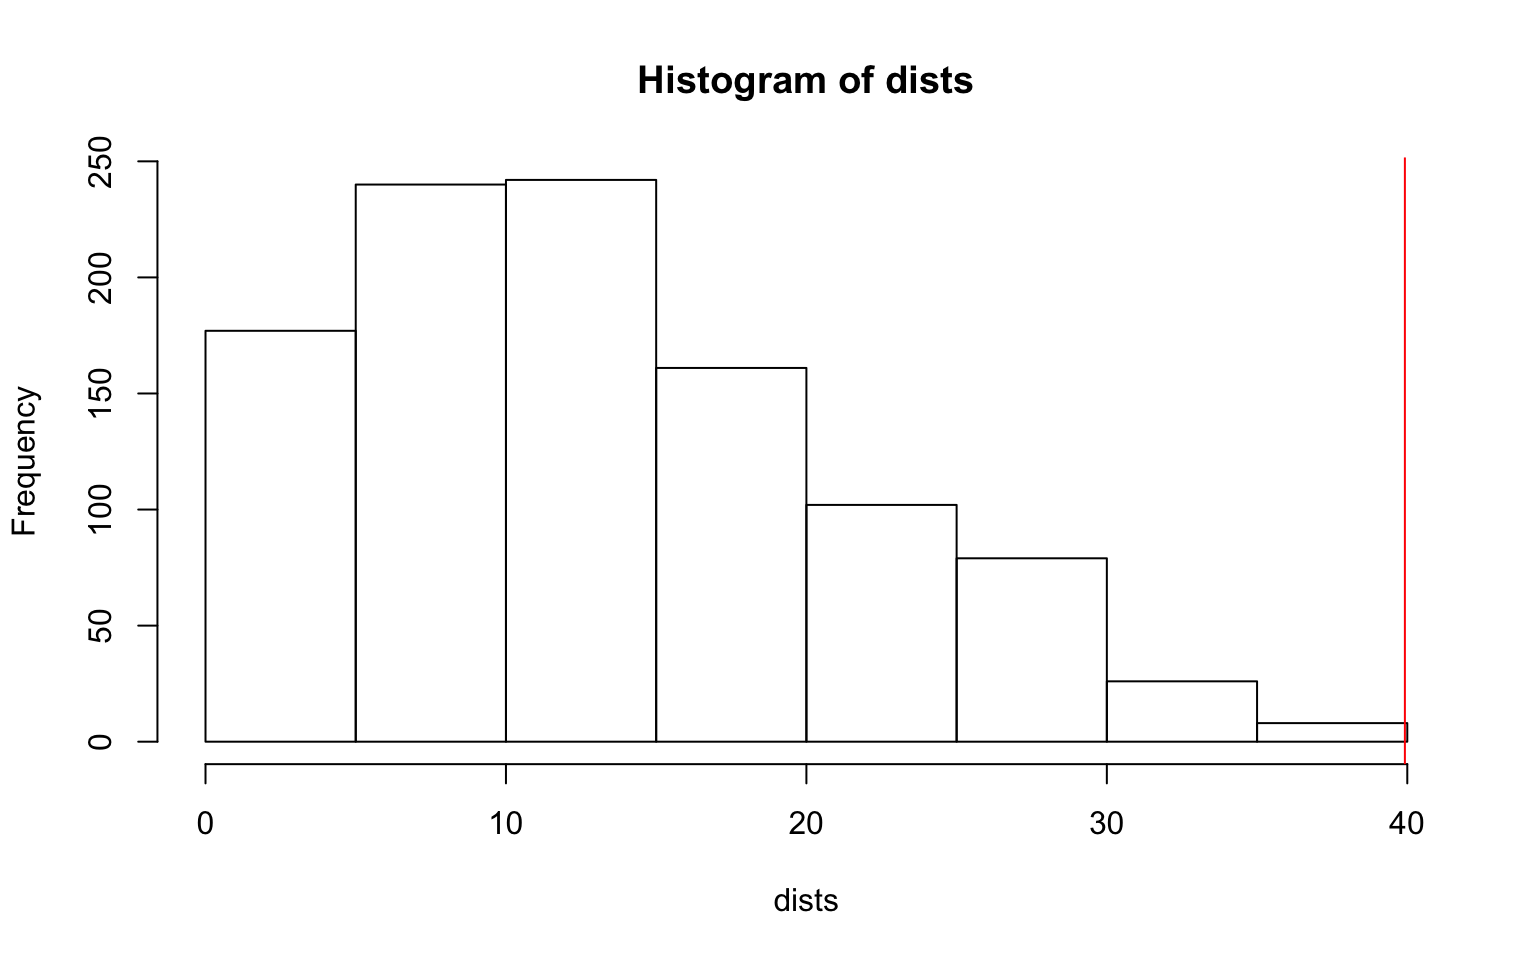
\includegraphics{project2_files/figure-latex/unnamed-chunk-3-1} \end{center}

I performed a randomization-test MANOVA -- a PERMANOVA because it allows
for differences in variance and isn't sensitive to outliers.

The null hypothesis: There are no differences in the centroids among
groups, given any differences in within group dispersions. Alternative
hypothesis: There are differences in the centroids among groups/ the
spread of the objects is different between the groups. A histogram with
the test statistic was plotted.

\begin{itemize}
\item
  \textbf{3. (35 pts)} Build a linear regression model predicting one of
  your response variables from at least 2 other variables, including
  their interaction. Mean-center any numeric variables involved in the
  interaction.

  \begin{itemize}
  \tightlist
  \item
    Interpret the coefficient estimates (do not discuss significance)
    (10)
  \item
    Plot the regression using \texttt{ggplot()}. If your interaction is
    numeric by numeric, refer to code near the end of WS15 to make the
    plot. If you have 3 or more predictors, just chose two to plot for
    convenience. (8)
  \item
    Check assumptions of linearity, normality, and homoskedasticity
    either graphically or using a hypothesis test (4)
  \item
    Regardless, recompute regression results with robust standard errors
    via \texttt{coeftest(...,\ vcov=vcovHC(...))}. Discuss significance
    of results, including any changes from before/after robust SEs if
    applicable. (8)
  \item
    What proportion of the variation in the outcome does your model
    explain? (4)
  \end{itemize}
\end{itemize}

\begin{Shaded}
\begin{Highlighting}[]
\KeywordTok{library}\NormalTok{(lmtest)}
\KeywordTok{library}\NormalTok{(sandwich)}
\NormalTok{together}\OperatorTok{$}\NormalTok{gsp_c <-}\StringTok{ }\NormalTok{together}\OperatorTok{$}\NormalTok{gsp }\OperatorTok{-}\StringTok{ }\KeywordTok{mean}\NormalTok{(together}\OperatorTok{$}\NormalTok{gsp)}
\NormalTok{fit1<-}\KeywordTok{lm}\NormalTok{(Value}\OperatorTok{~}\NormalTok{gsp_c}\OperatorTok{*}\StringTok{`}\DataTypeTok{Political Party}\StringTok{`}\NormalTok{ , }\DataTypeTok{data=}\NormalTok{together)}
\KeywordTok{summary}\NormalTok{(fit1)}
\end{Highlighting}
\end{Shaded}

\begin{verbatim}
##
## Call:
## lm(formula = Value ~ gsp_c * `Political Party`, data =
together)
##
## Residuals:
## Min 1Q Median 3Q Max
## -7.3824 -1.3208 -0.2833 2.0177 6.5527
##
## Coefficients:
## Estimate Std. Error t value Pr(>|t|)
## (Intercept) 2.838e+01 6.514e-01 43.570 <2e-16 ***
## gsp_c -3.659e-06 8.249e-06 -0.444 0.6596
## `Political Party`Republican 2.320e+00 9.167e-01 2.531
0.0152 *
## gsp_c:`Political Party`Republican 2.125e-06 1.667e-05
0.127 0.8992
## ---
## Signif. codes: 0 '***' 0.001 '**' 0.01 '*' 0.05 '.' 0.1
' ' 1
##
## Residual standard error: 2.997 on 42 degrees of freedom
## Multiple R-squared: 0.1524, Adjusted R-squared: 0.0919
## F-statistic: 2.518 on 3 and 42 DF, p-value: 0.07103
\end{verbatim}

\begin{Shaded}
\begin{Highlighting}[]
\KeywordTok{ggplot}\NormalTok{(together,}\KeywordTok{aes}\NormalTok{(gsp_c,Value)) }\OperatorTok{+}\StringTok{ }\KeywordTok{geom_point}\NormalTok{(}\KeywordTok{aes}\NormalTok{(}\DataTypeTok{color=}\StringTok{`}\DataTypeTok{Political Party}\StringTok{`}\NormalTok{)) }\OperatorTok{+}\StringTok{ }\KeywordTok{geom_smooth}\NormalTok{(}\DataTypeTok{method=}\StringTok{"lm"}\NormalTok{)}
\end{Highlighting}
\end{Shaded}

\begin{center}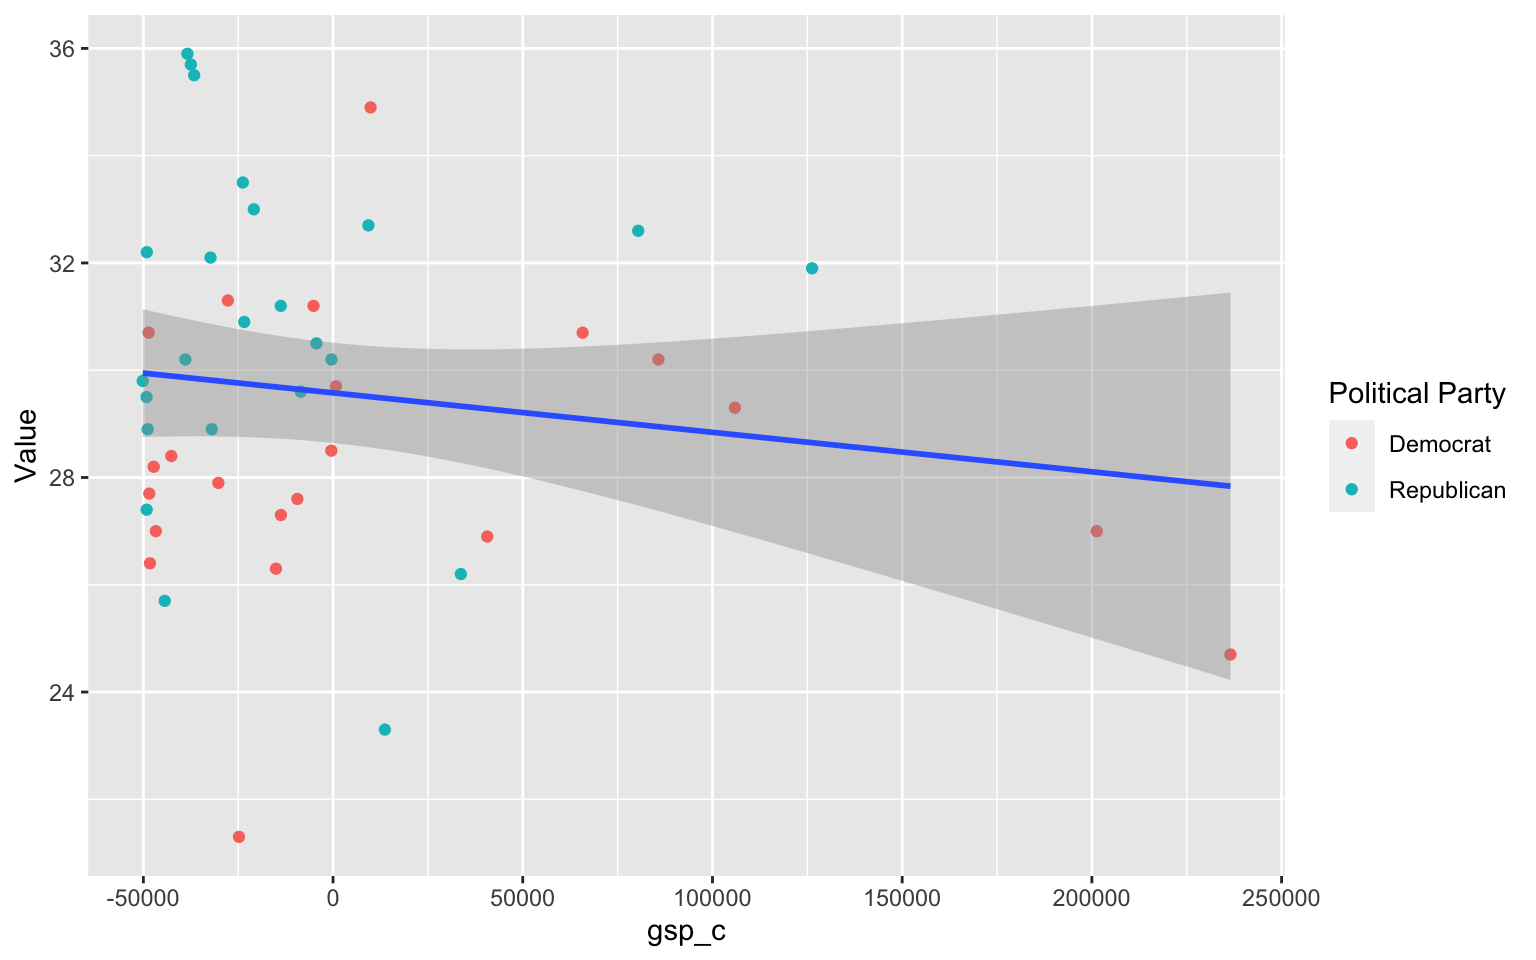
\includegraphics{project2_files/figure-latex/unnamed-chunk-4-1} \end{center}

\begin{Shaded}
\begin{Highlighting}[]
\CommentTok{#checking assumptions}
\NormalTok{resids<-fit1}\OperatorTok{$}\NormalTok{residuals}
\NormalTok{fitvals<-fit1}\OperatorTok{$}\NormalTok{fitted.values}
\KeywordTok{ggplot}\NormalTok{()}\OperatorTok{+}\KeywordTok{geom_point}\NormalTok{(}\KeywordTok{aes}\NormalTok{(fitvals,resids))}\OperatorTok{+}\KeywordTok{geom_hline}\NormalTok{(}\DataTypeTok{yintercept=}\DecValTok{0}\NormalTok{, }\DataTypeTok{color=}\StringTok{'red'}\NormalTok{)}
\end{Highlighting}
\end{Shaded}

\begin{center}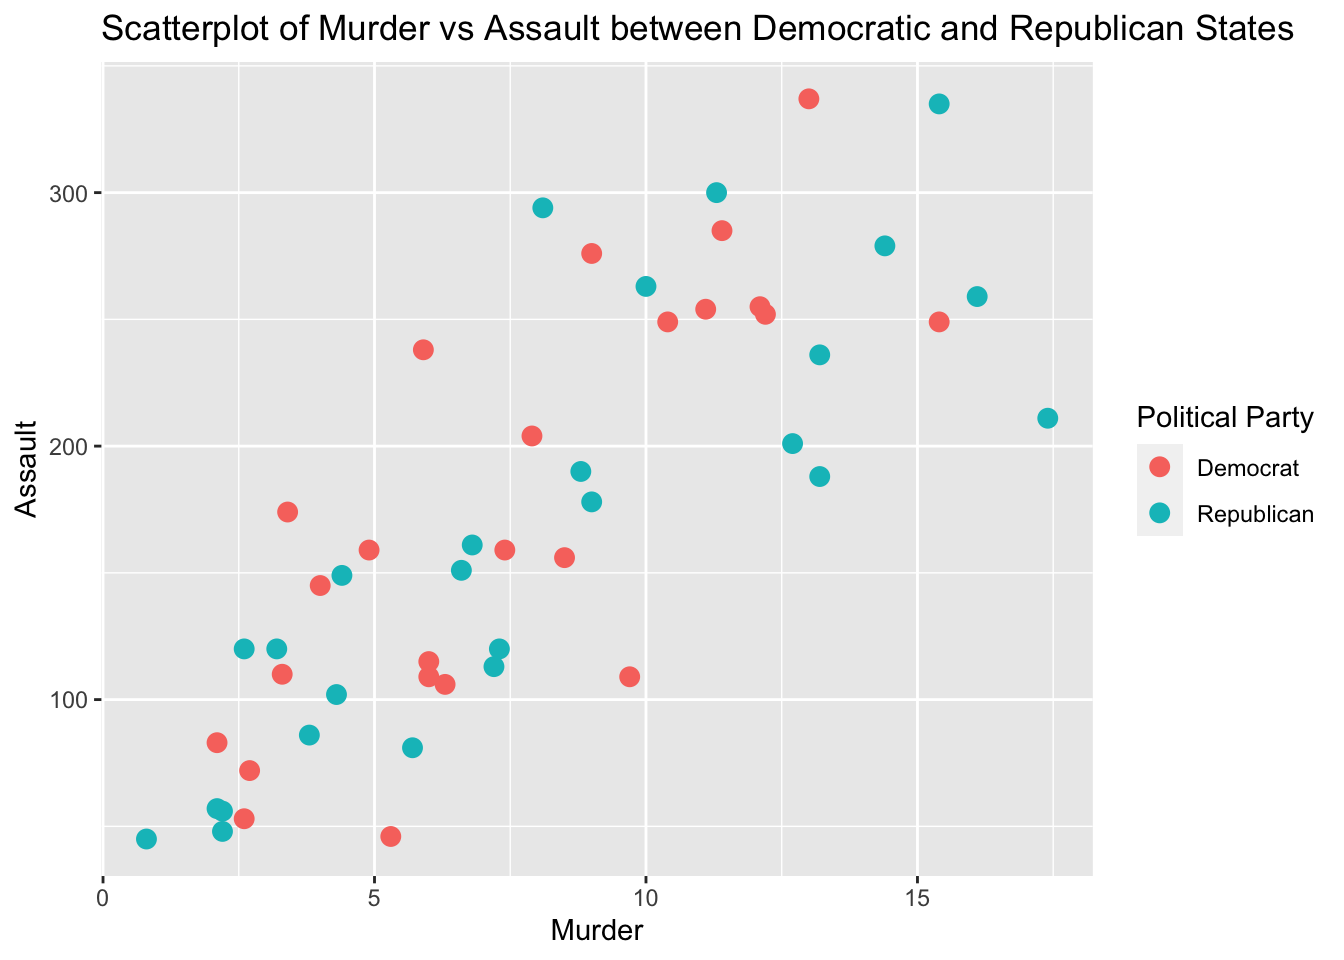
\includegraphics{project2_files/figure-latex/unnamed-chunk-4-2} \end{center}

\begin{Shaded}
\begin{Highlighting}[]
\KeywordTok{ggplot}\NormalTok{()}\OperatorTok{+}\KeywordTok{geom_histogram}\NormalTok{(}\KeywordTok{aes}\NormalTok{(resids),}\DataTypeTok{bins=}\DecValTok{10}\NormalTok{)}
\end{Highlighting}
\end{Shaded}

\begin{center}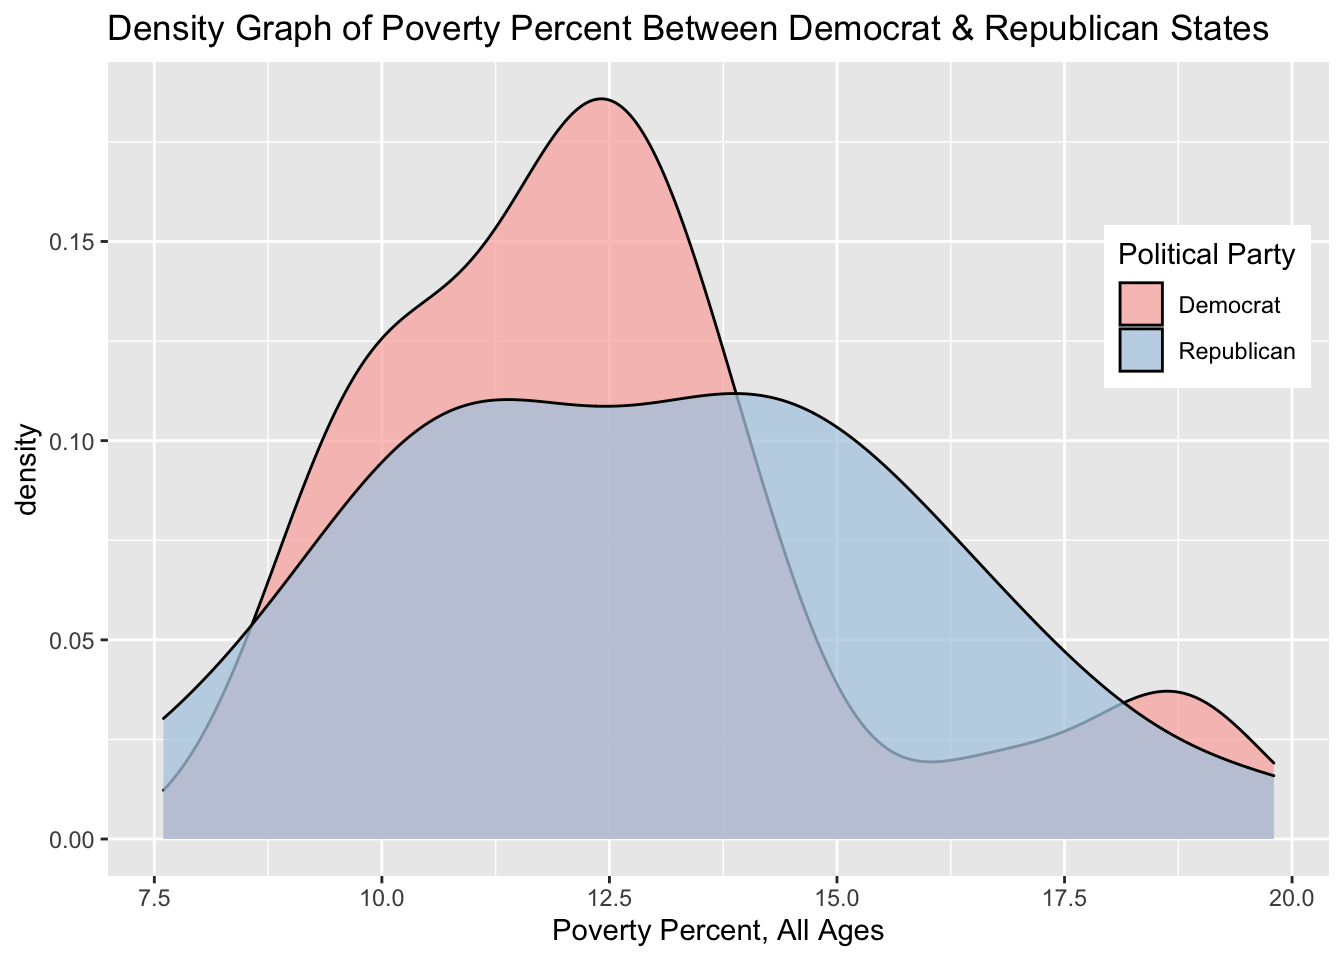
\includegraphics{project2_files/figure-latex/unnamed-chunk-4-3} \end{center}

\begin{Shaded}
\begin{Highlighting}[]
\KeywordTok{ggplot}\NormalTok{()}\OperatorTok{+}\KeywordTok{geom_qq}\NormalTok{(}\KeywordTok{aes}\NormalTok{(}\DataTypeTok{sample=}\NormalTok{resids))}\OperatorTok{+}\KeywordTok{geom_qq_line}\NormalTok{(}\KeywordTok{aes}\NormalTok{(}\DataTypeTok{sample=}\NormalTok{resids), }\DataTypeTok{color=}\StringTok{'red'}\NormalTok{)}
\end{Highlighting}
\end{Shaded}

\begin{center}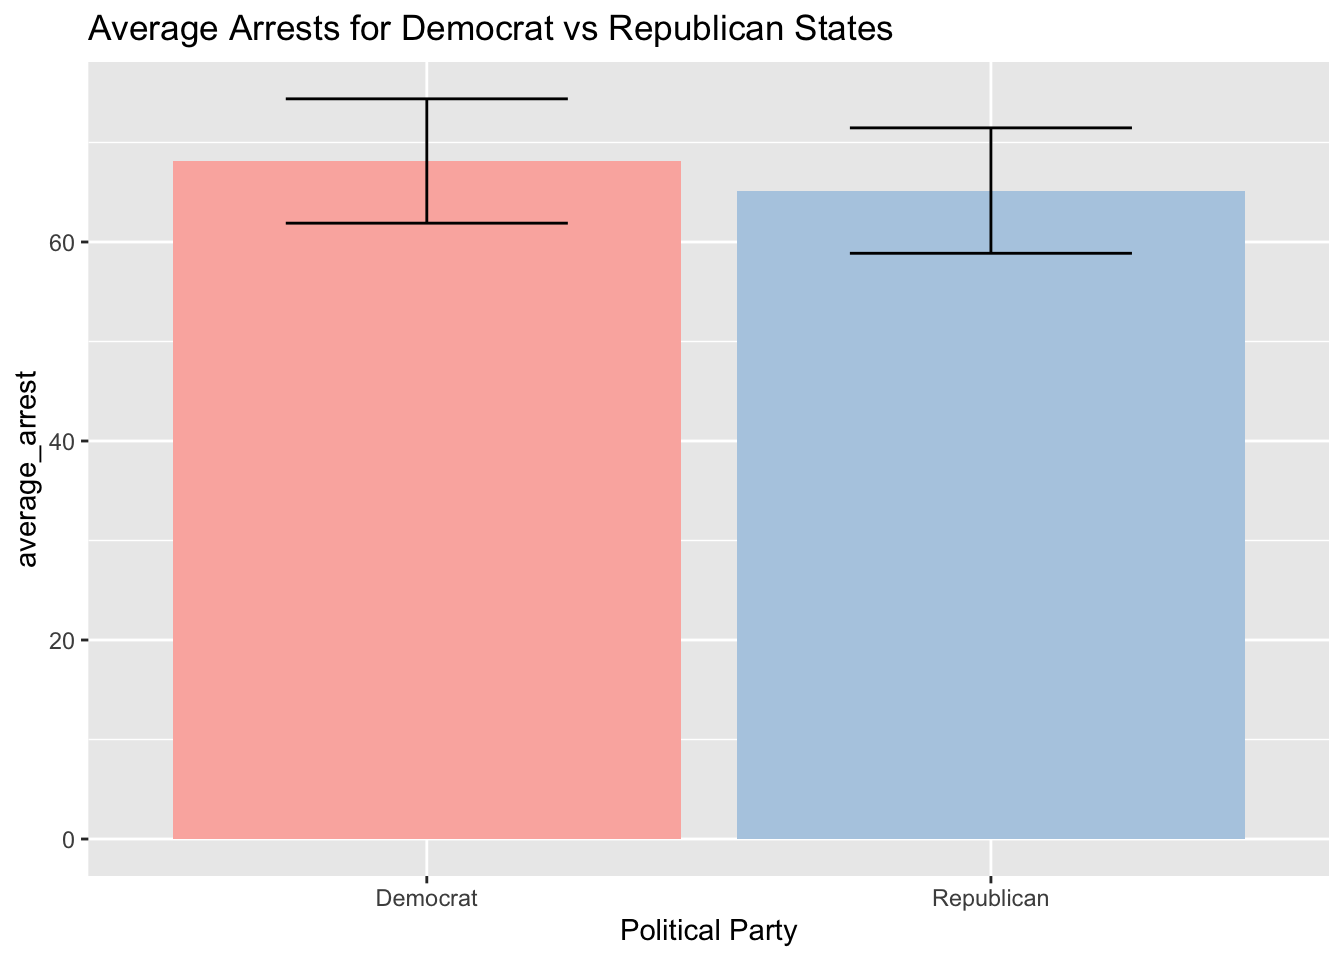
\includegraphics{project2_files/figure-latex/unnamed-chunk-4-4} \end{center}

\begin{Shaded}
\begin{Highlighting}[]
\CommentTok{#robust standard errors}
\KeywordTok{coeftest}\NormalTok{(fit1, }\DataTypeTok{vcov =} \KeywordTok{vcovHC}\NormalTok{(fit1))}
\end{Highlighting}
\end{Shaded}

\begin{verbatim}
##
## t test of coefficients:
##
## Estimate Std. Error t value Pr(>|t|)
## (Intercept) 2.8384e+01 6.2215e-01 45.6213 < 2e-16 ***
## gsp_c -3.6589e-06 9.0118e-06 -0.4060 0.68680
## `Political Party`Republican 2.3199e+00 9.5531e-01 2.4284
0.01953 *
## gsp_c:`Political Party`Republican 2.1253e-06 1.7725e-05
0.1199 0.90513
## ---
## Signif. codes: 0 '***' 0.001 '**' 0.01 '*' 0.05 '.' 0.1
' ' 1
\end{verbatim}

Predicted obesity levels for democratic states is 2.84e1, controlling
for an average gross state product.

Controlling for a state's political party, there is a decrease of
3.659e-6 in obesity levels for every 1 unit increase in gross state
product on average. Controlling for average gross state product, there
is an increase in 2.320 in obesity levels for republican states. The
slope for gsp on obesity levels is 2.125e-6 higher for republican states
compared to democratic states.

I checked assumptions by making a graph of residuals for
homoskedasticity, histogram for normality, and making a qqplot for
linearity. It appears that the dataset fits the assumptions.

After robust standard errors were computed, there were no changes in
significant p-values. My model explains 9.1\% of the proportion of
variation in the outcome (not that great\ldots{}).

\begin{itemize}
\tightlist
\item
  \textbf{4. (5 pts)} Rerun same regression model (with interaction),
  but this time compute bootstrapped standard errors. Discuss any
  changes you observe in SEs and p-values using these SEs compared to
  the original SEs and the robust SEs)
\end{itemize}

\begin{Shaded}
\begin{Highlighting}[]
\KeywordTok{library}\NormalTok{(dplyr)}
\NormalTok{samp_distn<-}\KeywordTok{replicate}\NormalTok{(}\DecValTok{5000}\NormalTok{, \{}
\NormalTok{boot_dat <-}\StringTok{ }\KeywordTok{sample_frac}\NormalTok{(together, }\DataTypeTok{replace=}\NormalTok{T) }\CommentTok{#bootstrap your data}
\NormalTok{fit1 <-}\StringTok{ }\KeywordTok{lm}\NormalTok{(Value}\OperatorTok{~}\NormalTok{gsp_c}\OperatorTok{*}\StringTok{`}\DataTypeTok{Political Party}\StringTok{`}\NormalTok{ , }\DataTypeTok{data=}\NormalTok{boot_dat) }\CommentTok{#fit model}
\KeywordTok{coef}\NormalTok{(fit1) }\CommentTok{#save coefs}
\NormalTok{\})}
\CommentTok{## Estimated SEs}
\NormalTok{samp_distn }\OperatorTok\StringTok{ }\NormalTok{t }\OperatorTok\StringTok{ }\NormalTok{as.data.frame }\OperatorTok\StringTok{ }\KeywordTok{summarize_all}\NormalTok{(sd)}
\end{Highlighting}
\end{Shaded}

\begin{verbatim}
## (Intercept) gsp_c `Political Party`Republican
gsp_c:`Political Party`Republican
## 1 0.6070209 9.515748e-06 0.9972755 2.211928e-05
\end{verbatim}

\begin{Shaded}
\begin{Highlighting}[]
\KeywordTok{summary}\NormalTok{(fit1)}
\end{Highlighting}
\end{Shaded}

\begin{verbatim}
##
## Call:
## lm(formula = Value ~ gsp_c * `Political Party`, data =
together)
##
## Residuals:
## Min 1Q Median 3Q Max
## -7.3824 -1.3208 -0.2833 2.0177 6.5527
##
## Coefficients:
## Estimate Std. Error t value Pr(>|t|)
## (Intercept) 2.838e+01 6.514e-01 43.570 <2e-16 ***
## gsp_c -3.659e-06 8.249e-06 -0.444 0.6596
## `Political Party`Republican 2.320e+00 9.167e-01 2.531
0.0152 *
## gsp_c:`Political Party`Republican 2.125e-06 1.667e-05
0.127 0.8992
## ---
## Signif. codes: 0 '***' 0.001 '**' 0.01 '*' 0.05 '.' 0.1
' ' 1
##
## Residual standard error: 2.997 on 42 degrees of freedom
## Multiple R-squared: 0.1524, Adjusted R-squared: 0.0919
## F-statistic: 2.518 on 3 and 42 DF, p-value: 0.07103
\end{verbatim}

With the bootstrapped standard errors, there were little changes in SEs
but the coefficients changed and all became significant. Comparing the
SEs, the intercept boostrapped SE decreased while the gsp\_c, political
party Republican, and the gsp\_c: Political Party Republican
coefficients boostrapped SEs increased.

\begin{itemize}
\item
  \textbf{5. (40 pts)} Perform a logistic regression predicting a binary
  categorical variable (if you don't have one, make/get one) from at
  least two explanatory variables (interaction not necessary).

  \begin{itemize}
  \tightlist
  \item
    Interpret coefficient estimates in context (10)
  \item
    Report a confusion matrix for your logistic regression (2)
  \item
    Compute and discuss the Accuracy, Sensitivity (TPR), Specificity
    (TNR), and Recall (PPV) of your model (5)
  \item
    Using ggplot, plot density of log-odds (logit) by your binary
    outcome variable (3)
  \item
    Generate an ROC curve (plot) and calculate AUC (either manually or
    with a package); interpret (10)
  \item
    Perform 10-fold (or repeated random sub-sampling) CV and report
    average out-of-sample Accuracy, Sensitivity, and Recall (10)
  \end{itemize}
\end{itemize}

\begin{Shaded}
\begin{Highlighting}[]
\NormalTok{data<-togetherbinary}\OperatorTok\KeywordTok{mutate}\NormalTok{(}\DataTypeTok{y=}\KeywordTok{ifelse}\NormalTok{(Death}\OperatorTok{==}\StringTok{"yes"}\NormalTok{,}\DecValTok{1}\NormalTok{,}\DecValTok{0}\NormalTok{))}
\NormalTok{fit2<-}\KeywordTok{glm}\NormalTok{(y}\OperatorTok{~}\StringTok{`}\DataTypeTok{Poverty Percent, All Ages}\StringTok{`}\OperatorTok{+}\StringTok{`}\DataTypeTok{Political Party}\StringTok{`}\NormalTok{,}\DataTypeTok{data=}\NormalTok{data,}\DataTypeTok{family=}\StringTok{"binomial"}\NormalTok{)}
\KeywordTok{coeftest}\NormalTok{(fit2)}
\end{Highlighting}
\end{Shaded}

\begin{verbatim}
##
## z test of coefficients:
##
## Estimate Std. Error z value Pr(>|z|)
## (Intercept) -4.56654 1.93191 -2.3637 0.01809 *
## `Poverty Percent, All Ages` 0.33585 0.15113 2.2223
0.02626 *
## `Political Party`Republican 1.43774 0.69006 2.0835
0.03721 *
## ---
## Signif. codes: 0 '***' 0.001 '**' 0.01 '*' 0.05 '.' 0.1
' ' 1
\end{verbatim}

\begin{Shaded}
\begin{Highlighting}[]
\NormalTok{prob<-}\KeywordTok{predict}\NormalTok{(fit2,}\DataTypeTok{type=}\StringTok{"response"}\NormalTok{)}
\NormalTok{pred<-}\StringTok{ }\KeywordTok{ifelse}\NormalTok{(prob}\OperatorTok{>}\NormalTok{.}\DecValTok{5}\NormalTok{,}\DecValTok{1}\NormalTok{,}\DecValTok{0}\NormalTok{)}
\KeywordTok{table}\NormalTok{(}\DataTypeTok{truth=}\NormalTok{data}\OperatorTok{$}\NormalTok{y, }\DataTypeTok{prediction=}\NormalTok{pred)}\OperatorTok\NormalTok{addmargins}
\end{Highlighting}
\end{Shaded}

\begin{verbatim}
##      prediction
## truth  0  1 Sum
##   0   12  7  19
##   1    8 19  27
##   Sum 20 26  46
\end{verbatim}

\begin{Shaded}
\begin{Highlighting}[]
\CommentTok{#accuracy = proportion of correctly identified cases}
\NormalTok{(}\DecValTok{19}\OperatorTok{+}\DecValTok{12}\NormalTok{)}\OperatorTok{/}\DecValTok{46}
\end{Highlighting}
\end{Shaded}

\begin{verbatim}
## [1] 0.673913
\end{verbatim}

\begin{Shaded}
\begin{Highlighting}[]
\CommentTok{#sensitivity (tpr) }
\DecValTok{19}\OperatorTok{/}\DecValTok{27}
\end{Highlighting}
\end{Shaded}

\begin{verbatim}
## [1] 0.7037037
\end{verbatim}

\begin{Shaded}
\begin{Highlighting}[]
\CommentTok{#specificity (tnr) }
\DecValTok{12}\OperatorTok{/}\DecValTok{19}
\end{Highlighting}
\end{Shaded}

\begin{verbatim}
## [1] 0.6315789
\end{verbatim}

\begin{Shaded}
\begin{Highlighting}[]
\CommentTok{#recall (ppv)}
\DecValTok{19}\OperatorTok{/}\DecValTok{26}
\end{Highlighting}
\end{Shaded}

\begin{verbatim}
## [1] 0.7307692
\end{verbatim}

\begin{Shaded}
\begin{Highlighting}[]
\CommentTok{#ggplot for logodds}

\NormalTok{data}\OperatorTok{$}\NormalTok{logit<-}\KeywordTok{predict}\NormalTok{(fit2)}
\KeywordTok{ggplot}\NormalTok{(data,}\KeywordTok{aes}\NormalTok{(logit, }\DataTypeTok{fill=}\NormalTok{Death)) }\OperatorTok{+}\StringTok{ }\KeywordTok{geom_density}\NormalTok{(}\DataTypeTok{alpha=}\NormalTok{.}\DecValTok{3}\NormalTok{) }\OperatorTok{+}\StringTok{ }\KeywordTok{geom_vline}\NormalTok{(}\DataTypeTok{xintercept=}\DecValTok{0}\NormalTok{,}\DataTypeTok{lty=}\DecValTok{2}\NormalTok{)}
\end{Highlighting}
\end{Shaded}

\begin{center}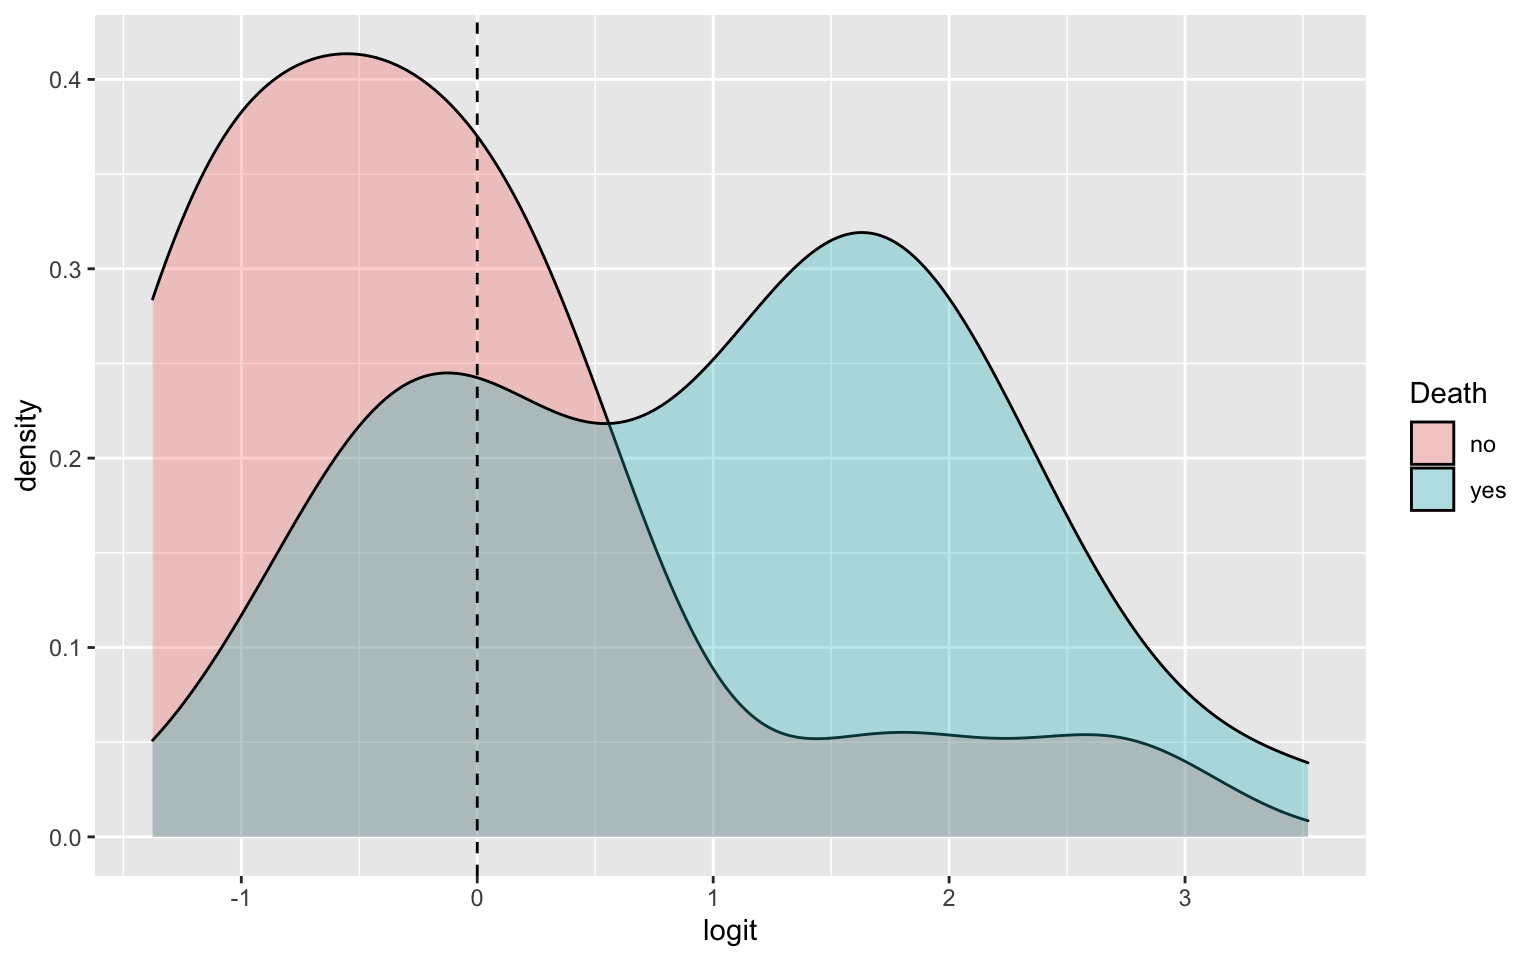
\includegraphics{project2_files/figure-latex/unnamed-chunk-6-1} \end{center}

\begin{Shaded}
\begin{Highlighting}[]
\CommentTok{#ROC AND AUC}
\NormalTok{sens<-}\ControlFlowTok{function}\NormalTok{(p,}\DataTypeTok{data=}\NormalTok{data, }\DataTypeTok{y=}\NormalTok{y) }\KeywordTok{mean}\NormalTok{(data[data}\OperatorTok{$}\NormalTok{y}\OperatorTok{==}\DecValTok{1}\NormalTok{,]}\OperatorTok{$}\NormalTok{prob}\OperatorTok{>}\NormalTok{p)}
\NormalTok{spec<-}\ControlFlowTok{function}\NormalTok{(p,}\DataTypeTok{data=}\NormalTok{data, }\DataTypeTok{y=}\NormalTok{y) }\KeywordTok{mean}\NormalTok{(data[data}\OperatorTok{$}\NormalTok{y}\OperatorTok{==}\DecValTok{0}\NormalTok{,]}\OperatorTok{$}\NormalTok{prob}\OperatorTok{<}\NormalTok{p)}
\NormalTok{sensitivity<-}\KeywordTok{sapply}\NormalTok{(}\KeywordTok{seq}\NormalTok{(}\DecValTok{0}\NormalTok{,}\DecValTok{1}\NormalTok{,.}\DecValTok{01}\NormalTok{),sens,data)}
\NormalTok{specificity<-}\KeywordTok{sapply}\NormalTok{(}\KeywordTok{seq}\NormalTok{(}\DecValTok{0}\NormalTok{,}\DecValTok{1}\NormalTok{,.}\DecValTok{01}\NormalTok{),spec,data)}
\NormalTok{ROC1<-}\KeywordTok{data.frame}\NormalTok{(sensitivity,specificity,}\DataTypeTok{cutoff=}\KeywordTok{seq}\NormalTok{(}\DecValTok{0}\NormalTok{,}\DecValTok{1}\NormalTok{,.}\DecValTok{01}\NormalTok{))}
\NormalTok{ROC1}\OperatorTok\KeywordTok{gather}\NormalTok{(key,rate,}\OperatorTok{-}\NormalTok{cutoff)}\OperatorTok\KeywordTok{ggplot}\NormalTok{(}\KeywordTok{aes}\NormalTok{(cutoff,rate,}\DataTypeTok{color=}\NormalTok{key))}\OperatorTok{+}\KeywordTok{geom_path}\NormalTok{()}\OperatorTok{+}
\KeywordTok{geom_vline}\NormalTok{(}\DataTypeTok{xintercept=}\KeywordTok{c}\NormalTok{(.}\DecValTok{1}\NormalTok{,.}\DecValTok{5}\NormalTok{,.}\DecValTok{9}\NormalTok{),}\DataTypeTok{lty=}\DecValTok{2}\NormalTok{,}\DataTypeTok{color=}\StringTok{"gray50"}\NormalTok{)}
\end{Highlighting}
\end{Shaded}

\begin{center}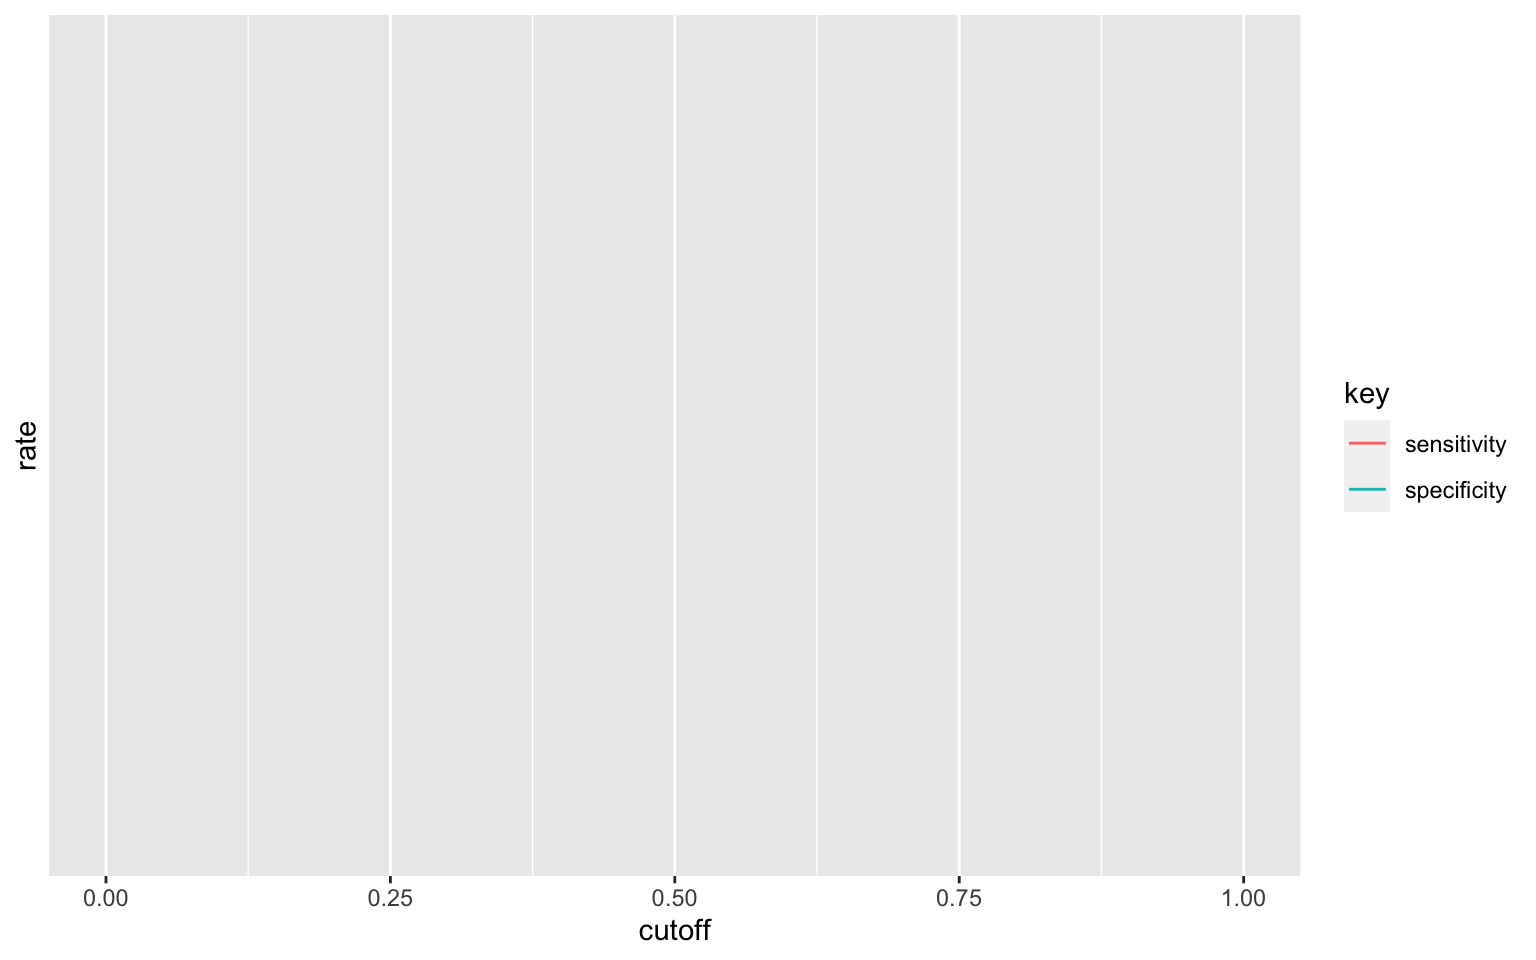
\includegraphics{project2_files/figure-latex/unnamed-chunk-6-2} \end{center}

\begin{Shaded}
\begin{Highlighting}[]
\NormalTok{ROC1}\OperatorTok{$}\NormalTok{TPR<-sensitivity}
\NormalTok{ROC1}\OperatorTok{$}\NormalTok{FPR<-}\DecValTok{1}\OperatorTok{-}\NormalTok{specificity}
\KeywordTok{library}\NormalTok{(plotROC)}
\NormalTok{ROCplot<-}\KeywordTok{ggplot}\NormalTok{(data)}\OperatorTok{+}\KeywordTok{geom_roc}\NormalTok{(}\KeywordTok{aes}\NormalTok{(}\DataTypeTok{d=}\NormalTok{data}\OperatorTok{$}\NormalTok{y,}\DataTypeTok{m=}\NormalTok{prob), }\DataTypeTok{n.cuts=}\DecValTok{0}\NormalTok{)}
\NormalTok{ROCplot}
\end{Highlighting}
\end{Shaded}

\begin{center}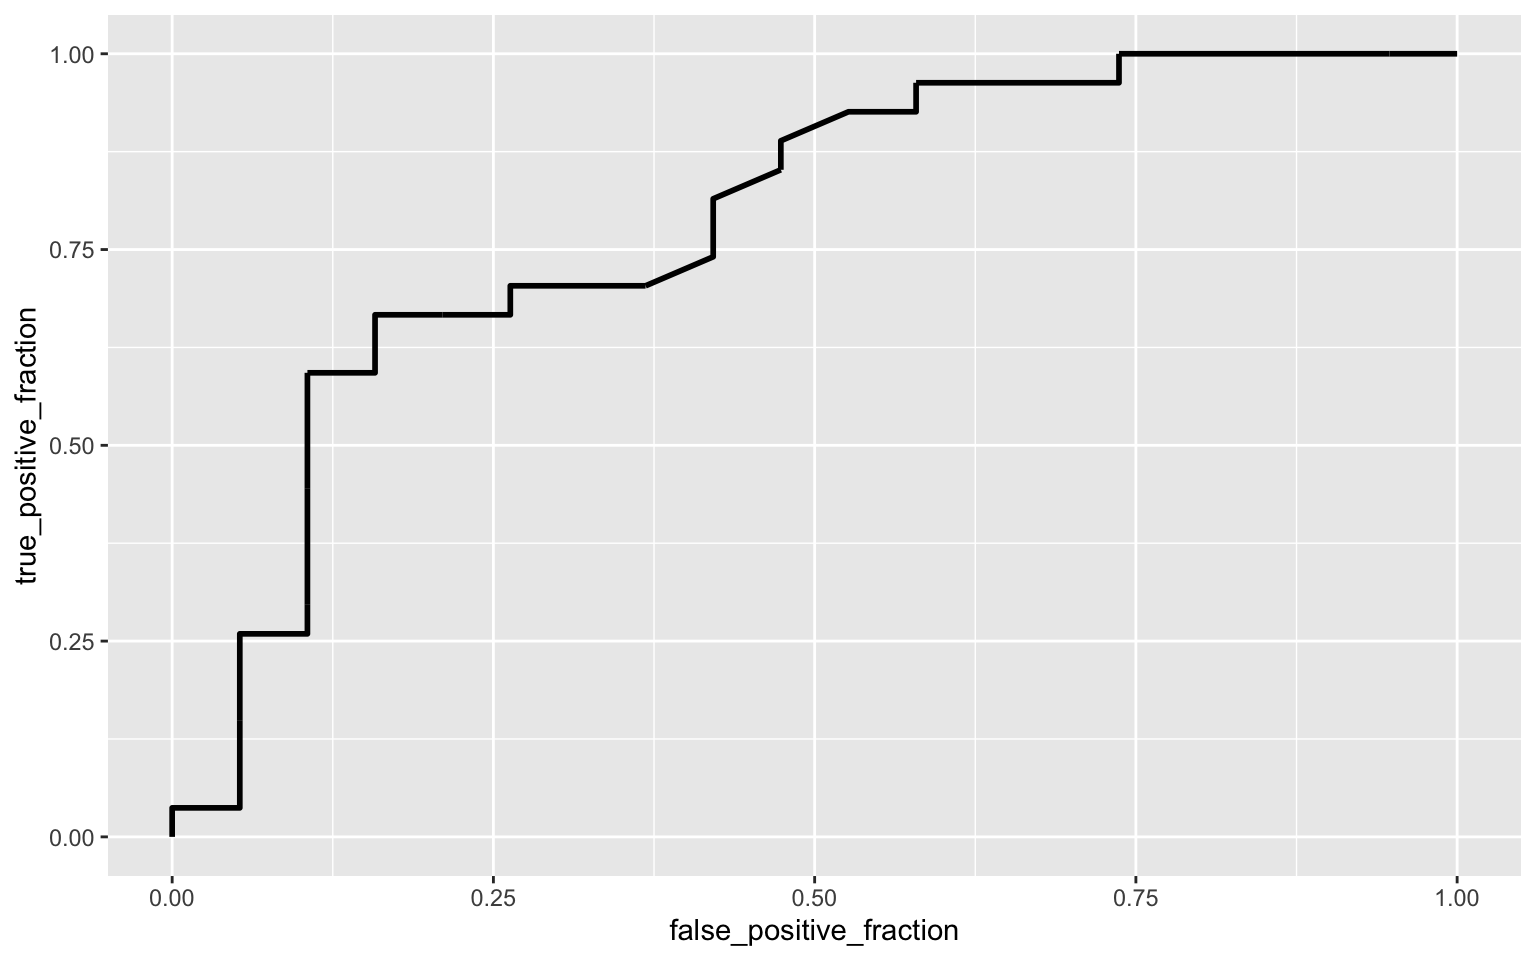
\includegraphics{project2_files/figure-latex/unnamed-chunk-6-3} \end{center}

\begin{Shaded}
\begin{Highlighting}[]
\CommentTok{#ACC,TPR,TNR,PPV,AUC}
\NormalTok{truth<-data}\OperatorTok{$}\NormalTok{y}
\NormalTok{class_diag<-}\ControlFlowTok{function}\NormalTok{(prob,truth)\{}

\NormalTok{tab<-}\KeywordTok{table}\NormalTok{(}\KeywordTok{factor}\NormalTok{(prob}\OperatorTok{>}\NormalTok{.}\DecValTok{5}\NormalTok{,}\DataTypeTok{levels=}\KeywordTok{c}\NormalTok{(}\StringTok{"FALSE"}\NormalTok{,}\StringTok{"TRUE"}\NormalTok{)),truth)}
\NormalTok{tab}
\NormalTok{acc=}\KeywordTok{sum}\NormalTok{(}\KeywordTok{diag}\NormalTok{(tab))}\OperatorTok{/}\KeywordTok{sum}\NormalTok{(tab)}
\NormalTok{sens=tab[}\DecValTok{2}\NormalTok{,}\DecValTok{2}\NormalTok{]}\OperatorTok{/}\KeywordTok{colSums}\NormalTok{(tab)[}\DecValTok{2}\NormalTok{]}
\NormalTok{spec=tab[}\DecValTok{1}\NormalTok{,}\DecValTok{1}\NormalTok{]}\OperatorTok{/}\KeywordTok{colSums}\NormalTok{(tab)[}\DecValTok{1}\NormalTok{]}
\NormalTok{ppv=tab[}\DecValTok{2}\NormalTok{,}\DecValTok{2}\NormalTok{]}\OperatorTok{/}\KeywordTok{rowSums}\NormalTok{(tab)[}\DecValTok{2}\NormalTok{]}

\ControlFlowTok{if}\NormalTok{(}\KeywordTok{is.numeric}\NormalTok{(truth)}\OperatorTok{==}\OtherTok{FALSE} \OperatorTok{&}\StringTok{ }\KeywordTok{is.logical}\NormalTok{(truth)}\OperatorTok{==}\OtherTok{FALSE}\NormalTok{) truth<-}\KeywordTok{as.numeric}\NormalTok{(truth)}\OperatorTok{-}\DecValTok{1}

\CommentTok{#CALCULATE EXACT AUC}
\NormalTok{ord<-}\KeywordTok{order}\NormalTok{(prob, }\DataTypeTok{decreasing=}\OtherTok{TRUE}\NormalTok{)}
\NormalTok{prob <-}\StringTok{ }\NormalTok{prob[ord]; truth <-}\StringTok{ }\NormalTok{truth[ord]}

\NormalTok{TPR=}\KeywordTok{cumsum}\NormalTok{(truth)}\OperatorTok{/}\KeywordTok{max}\NormalTok{(}\DecValTok{1}\NormalTok{,}\KeywordTok{sum}\NormalTok{(truth)) }
\NormalTok{FPR=}\KeywordTok{cumsum}\NormalTok{(}\OperatorTok{!}\NormalTok{truth)}\OperatorTok{/}\KeywordTok{max}\NormalTok{(}\DecValTok{1}\NormalTok{,}\KeywordTok{sum}\NormalTok{(}\OperatorTok{!}\NormalTok{truth))}

\NormalTok{dup<-}\KeywordTok{c}\NormalTok{(prob[}\OperatorTok{-}\DecValTok{1}\NormalTok{]}\OperatorTok{>=}\NormalTok{prob[}\OperatorTok{-}\KeywordTok{length}\NormalTok{(prob)], }\OtherTok{FALSE}\NormalTok{)}
\NormalTok{TPR<-}\KeywordTok{c}\NormalTok{(}\DecValTok{0}\NormalTok{,TPR[}\OperatorTok{!}\NormalTok{dup],}\DecValTok{1}\NormalTok{); FPR<-}\KeywordTok{c}\NormalTok{(}\DecValTok{0}\NormalTok{,FPR[}\OperatorTok{!}\NormalTok{dup],}\DecValTok{1}\NormalTok{)}

\NormalTok{n <-}\StringTok{ }\KeywordTok{length}\NormalTok{(TPR)}
\NormalTok{auc<-}\StringTok{ }\KeywordTok{sum}\NormalTok{( ((TPR[}\OperatorTok{-}\DecValTok{1}\NormalTok{]}\OperatorTok{+}\NormalTok{TPR[}\OperatorTok{-}\NormalTok{n])}\OperatorTok{/}\DecValTok{2}\NormalTok{) }\OperatorTok{*}\StringTok{ }\NormalTok{(FPR[}\OperatorTok{-}\DecValTok{1}\NormalTok{]}\OperatorTok{-}\NormalTok{FPR[}\OperatorTok{-}\NormalTok{n]) )}

\KeywordTok{data.frame}\NormalTok{(acc,sens,spec,ppv,auc)}
\NormalTok{\}}

\KeywordTok{class_diag}\NormalTok{(prob,truth)}
\end{Highlighting}
\end{Shaded}

\begin{verbatim}
##        acc      sens      spec       ppv       auc
## 1 0.673913 0.7037037 0.6315789 0.7307692 0.7846004
\end{verbatim}

\begin{Shaded}
\begin{Highlighting}[]
\KeywordTok{library}\NormalTok{(slackr)}
\CommentTok{##10fold}
\KeywordTok{set.seed}\NormalTok{(}\DecValTok{1234}\NormalTok{)}
\NormalTok{k=}\DecValTok{5}

\NormalTok{data1<-data[}\KeywordTok{sample}\NormalTok{(}\KeywordTok{nrow}\NormalTok{(data)),] }\CommentTok{#put dataset in random order}
\NormalTok{folds<-}\KeywordTok{cut}\NormalTok{(}\KeywordTok{seq}\NormalTok{(}\DecValTok{1}\OperatorTok{:}\KeywordTok{nrow}\NormalTok{(data)),}\DataTypeTok{breaks=}\NormalTok{k,}\DataTypeTok{labels=}\NormalTok{F) }\CommentTok{#create folds}

\NormalTok{diags<-}\OtherTok{NULL}
\ControlFlowTok{for}\NormalTok{(i }\ControlFlowTok{in} \DecValTok{1}\OperatorTok{:}\NormalTok{k)\{          }\CommentTok{# FOR EACH OF 10 FOLDS}
\NormalTok{  train<-data1[folds}\OperatorTok{!=}\NormalTok{i,] }\CommentTok{# CREATE TRAINING SET}
\NormalTok{  test<-data1[folds}\OperatorTok{==}\NormalTok{i,]  }\CommentTok{# CREATE }\AlertTok{TESTING}\CommentTok{ SET}
\NormalTok{  truth<-test}\OperatorTok{$}\NormalTok{y}
\NormalTok{  train}
\NormalTok{  fit<-}\KeywordTok{glm}\NormalTok{(y}\OperatorTok{~}\StringTok{`}\DataTypeTok{Poverty Percent, All Ages}\StringTok{`}\OperatorTok{+}\StringTok{`}\DataTypeTok{Political Party}\StringTok{`}\NormalTok{,}\DataTypeTok{data=}\NormalTok{train,}\DataTypeTok{family=}\StringTok{"binomial"}\NormalTok{)}
\NormalTok{  prob<-}\StringTok{ }\KeywordTok{predict}\NormalTok{(fit, }\DataTypeTok{newdata=}\NormalTok{test, }\DataTypeTok{type=}\StringTok{"response"}\NormalTok{)}
  
\NormalTok{  diags<-}\KeywordTok{rbind}\NormalTok{(diags,}\KeywordTok{class_diag}\NormalTok{(prob,truth)) }\CommentTok{#CV DIAGNOSTICS FOR EACH FOLD}
\NormalTok{\}}
\KeywordTok{summarize_all}\NormalTok{(diags,mean)}
\end{Highlighting}
\end{Shaded}

\begin{verbatim}
##         acc      sens spec       ppv       auc
## 1 0.6511111 0.6447619 0.63 0.7047619 0.7557143
\end{verbatim}

Intercept: Odds of death penalty for a democratic state, controlling for
poverty percentage is -4.56654. Poverty Percent, All Ages: Controlling
for political party, for every one increase in poverty percentage, odds
of the state having a death penalty increases by a factor or .33585.
Political party, republican: Controlling for poverty percentage, for
everyone one increase in a state being republican, the odds of the state
having a death penalty increases by 1.43774. Reported confusion matrix:

prediction truth 0 1 Sum 0 12 7 19 1 8 19 27 Sum 20 26 46

For my model, the accuracy (proportion of correctly identified cases) is
0.673913. The sensitivity (true positive rate) is 0.7037037. The
specificity (true negative rate) is 0.6315789. The recall is 0.7307692.

A ROC plot was generated and the AUC was calculated to be .7846004,
which is fair, and tells us the probability that a randomly selected y=1
has a higher predicted probability than a randomly selected y=0.

A 10-fold CV was performed. The accuracy was .67, the sensitivity was
.725, the recall was .7167, and the auc was .751.

\begin{itemize}
\tightlist
\item
  \textbf{6. (10 pts)} Choose one variable you want to predict (can be
  one you used from before; either binary or continuous) and run a LASSO
  regression inputting all the rest of your variables as predictors.
  Choose lambda to give the simplest model whose accuracy is near that
  of the best (i.e., \texttt{lambda.1se}). Discuss which variables are
  retained. Perform 10-fold CV using this model: if response in binary,
  compare model's out-of-sample accuracy to that of your logistic
  regression in part 5; if response is numeric, compare the residual
  standard error (at the bottom of the summary output, aka RMSE): lower
  is better fit!
\end{itemize}

\begin{Shaded}
\begin{Highlighting}[]
\KeywordTok{library}\NormalTok{(glmnet)}
\KeywordTok{set.seed}\NormalTok{(}\DecValTok{1234}\NormalTok{)}
\NormalTok{data1<-data}\OperatorTok\KeywordTok{select}\NormalTok{(}\OperatorTok{-}\NormalTok{State, }\OperatorTok{-}\NormalTok{year,}\OperatorTok{-}\NormalTok{Class,}\OperatorTok{-}\NormalTok{logit,}\OperatorTok{-}\StringTok{`}\DataTypeTok{Political Party}\StringTok{`}\NormalTok{,}\OperatorTok{-}\NormalTok{Short_Desc)}
\NormalTok{data2<-data1}\OperatorTok\KeywordTok{na.omit}\NormalTok{()}\OperatorTok\KeywordTok{as.matrix}\NormalTok{()}
\NormalTok{x<-}\KeywordTok{model.matrix}\NormalTok{(y}\OperatorTok{~}\NormalTok{.,}\DataTypeTok{data=}\NormalTok{data1)}
\KeywordTok{scale}\NormalTok{(x)}
\end{Highlighting}
\end{Shaded}

\begin{verbatim}
## (Intercept) Murder Assault Rape `Poverty Percent, All
Ages` pcap
## 1 NaN 1.202189712 0.74581096 0.014038290 1.428511558
-0.26581193
## 2 NaN 0.051031727 1.46054647 1.105152283 0.445024111
-0.44195720
## 3 NaN 0.209033803 0.17895177 -0.175236586 1.428511558
-0.55914326
## 4 NaN 0.254177253 1.23873200 2.173998643 -0.028506883
4.11518394
## 5 NaN 0.005888276 0.35147413 1.962456134 -1.157696174
-0.40990008
## 6 NaN -1.032411084 -0.80689031 -1.110477151 -0.939143408
-0.21463675
## 7 NaN -0.445546228 0.77045701 -0.587187787 -0.247059649
-0.69376067
## 8 NaN 1.698767667 1.96579053 1.205356629 0.299322267
0.35973568
## 9 NaN 2.150202171 0.43773531 0.526193838 0.590725955
-0.09696489
## 10 NaN -1.190413160 -0.68366005 -0.765328847
-0.429186954 -0.72993713
## 11 NaN 0.570181406 0.90601030 0.325785145 -0.283485110
1.23193722
## 12 NaN -0.152113800 -0.76992123 -0.008229342 0.044344039
-0.01578383
## 13 NaN -1.280700061 -1.47233371 -1.088209519
-0.611314259 -0.28045858
## 14 NaN -0.422974503 -0.74527518 -0.342243830
-0.356336032 -0.42220533
## 15 NaN 1.698767667 0.90601030 0.125376453 2.120595317
-0.08256150
## 16 NaN -1.303271786 -1.13961201 -1.477893088
-0.465612415 -0.71035159
## 17 NaN 0.773326933 1.53448462 0.748870163 -1.376248940
-0.05865330
## 18 NaN -0.784122106 -0.32629230 -0.531518706
-1.048419791 0.07706136
## 19 NaN 0.953900735 0.97994846 1.561638749 0.408598650
0.88885144
## 20 NaN -1.167841435 -1.27516529 -0.687392134
-1.194121635 0.03917877
## 21 NaN 1.856769743 1.02924056 -0.442448176 2.521275388
-0.46108222
## 22 NaN 0.254177253 0.03107546 0.793405428 0.117194962
-0.05798249
## 23 NaN -0.422974503 -0.81921333 -0.520384890 0.007918578
-0.67484520
## 24 NaN -0.806693831 -0.90547452 -0.509251074
-0.684165181 -0.47173850
## 25 NaN 0.976472460 0.94297938 2.775224720 0.080769501
-0.71443539
## 26 NaN -1.303271786 -1.46001068 -1.288618211
-1.922630855 -0.73646600
## 27 NaN -0.106970350 -0.20306204 -0.253173300
-1.230547096 0.21553689
## 28 NaN 0.795898659 1.34963923 1.227624261 2.157020778
-0.63510994
## 29 NaN 0.728183483 0.96762543 0.559595286 0.299322267
3.58255882
## 30 NaN 1.157046262 1.99043658 -0.553786339 0.445024111
-0.16779412
## 31 NaN -1.596704214 -1.60788699 -1.533562169
-0.829867025 -0.70821718
## 32 NaN -0.129542075 -0.68366005 0.036305923 0.335747728
1.05125240
## 33 NaN -0.287544152 -0.30164624 -0.119567505 0.954980565
-0.43336096
## 34 NaN -0.671263480 -0.20306204 0.915877406 -0.137783266
-0.42172504
## 35 NaN -0.355259327 -0.85618241 -0.687392134
-0.247059649 1.26131039
## 36 NaN -1.009839358 -0.01821665 -1.422224006
-0.028506883 -0.70207701
## 37 NaN 1.473050415 1.27570108 0.158777901 0.845704182
-0.51684825
## 38 NaN -0.919552457 -1.10264293 -0.921202275 0.007918578
-0.70539585
## 39 NaN 1.202189712 0.15430572 0.648665816 0.845704182
-0.02839353
## 40 NaN 1.089331086 0.31450505 0.492792389 0.736427799
1.29955641
## 41 NaN -1.054982809 -0.68366005 0.203313166 -1.376248940
-0.61302913
## 42 NaN 0.141318627 -0.24003111 -0.041630791 -0.793441564
-0.02691894
## 43 NaN -0.874409007 -0.37558440 0.570729103 -0.939143408
0.17331808
## 44 NaN -0.490689678 -1.16425806 -1.310885844 1.647064324
-0.56479911
## 45 NaN -1.190413160 -1.50930279 -1.143878600
-0.647739720 0.05734027
## 46 NaN -0.242400701 -0.17841598 -0.609455420
-0.793441564 -0.73047677
## hwy water util pc gsp emp unemp
## 1 -0.22128096 -0.372020522 -0.258686249 -0.205490645
-0.371105216 -0.28812373 -0.63869885
## 2 -0.52968258 -0.397580115 -0.380180709 -0.463969034
-0.498858256 -0.53321963 -0.47129061
## 3 -0.64162665 -0.656101625 -0.460788805 -0.578259736
-0.599034992 -0.59143718 -0.47129061
## 4 3.88034956 4.317044098 4.073193091 2.898259911
3.691288499 3.48809960 1.95612896
## 5 -0.52771854 -0.246555987 -0.359735811 -0.462294303
-0.386914382 -0.40426775 -1.05721947
## 6 -0.26480831 -0.101972454 -0.202813507 -0.464022634
-0.234909177 -0.22804322 0.86797536
## 7 -0.82691588 -0.766397503 -0.563632008 -0.876837826
-0.758546819 -0.80981122 -0.05276999
## 8 0.41685334 0.310966529 0.322030446 0.327435142
0.525741097 0.66844888 -0.30388236
## 9 -0.14079717 -0.230027288 -0.031028429 -0.057070619
-0.068436947 0.10018735 -0.63869885
## 10 -0.79828801 -0.779067793 -0.646988934 -0.808880548
-0.762479602 -0.80265046 0.78427124
## 11 1.61606763 0.997641645 0.996309693 1.603342314
1.652951766 1.65133581 -0.47129061
## 12 -0.03392399 -0.046183701 0.004382935 0.403436389
0.145525204 0.23152614 -0.38758648
## 13 -0.06240416 -0.435280042 -0.374227084 -0.253833745
-0.365362104 -0.38953871 -1.47574008
## 14 -0.38250414 -0.433857811 -0.430429439 -0.284471821
-0.432656400 -0.50480946 -1.30833184
## 15 0.06138910 -0.104119320 -0.168551667 1.033414877
0.154358361 -0.26448740 1.11908773
## 16 -0.79531419 -0.703711201 -0.631366678 -0.808809756
-0.737556367 -0.74262816 1.03538361
## 17 -0.17112825 0.318604935 -0.078668414 -0.340409262
-0.132360286 -0.09251275 -0.97351534
## 18 -0.10338611 -0.098203273 0.237157302 -0.138648034
0.213287689 0.40932255 1.70501659
## 19 0.92328898 1.740759849 0.618670657 0.891144432
1.026609171 0.96285504 0.95167949
## 20 0.12070000 0.186962079 -0.053173578 -0.028350798
-0.146764886 -0.11312177 -0.22017824
## 21 -0.47437937 -0.593545109 -0.402514012 -0.521241608
-0.571255806 -0.54561996 -0.88981122
## 22 0.05216910 -0.086536115 -0.120903441 -0.013308758
-0.006558032 0.08161595 -0.80610710
## 23 -0.65297200 -0.745631854 -0.647481980 -0.705817423
-0.753178257 -0.81866029 1.37020010
## 24 -0.58142224 -0.561339426 -0.360494606 -0.584923872
-0.607477991 -0.63405243 -1.14092359
## 25 -0.82786490 -0.705703946 -0.617176175 -0.768243841
-0.755893750 -0.80678391 1.28649598
## 26 -0.83409956 -0.756003863 -0.641608011 -0.875353019
-0.766443598 -0.77581217 -0.63869885
## 27 0.29256147 0.342982941 0.125097999 0.302935523
0.634204770 0.65744576 0.78427124
## 28 -0.68895114 -0.632429326 -0.578166543 -0.599724815
-0.665158816 -0.74775131 0.86797536
## 29 2.79242257 2.619638889 4.219142048 2.159632827
3.141369875 3.20300824 0.61686299
## 30 -0.12675349 -0.178378144 -0.186111083 -0.007789224
0.011951021 0.22570439 -0.97351534
## 31 -0.75271911 -0.759510770 -0.641117713 -0.759864319
-0.766100260 -0.84212196 0.36575062
## 32 1.55686042 1.368943880 0.602154327 1.380315033
1.255163198 1.44524568 -0.30388236
## 33 -0.45283776 -0.436961843 -0.404442932 -0.170460242
-0.325800174 -0.45322871 -0.38758648
## 34 -0.41219101 -0.349754231 -0.431427204 -0.504425121
-0.471828172 -0.47401237 0.53315887
## 35 1.53109011 1.135687243 1.072014804 1.384435114
1.338407116 1.67438997 0.11463826
## 36 -0.82132438 -0.690721855 -0.602103960 -0.892673139
-0.729019730 -0.73616601 1.28649598
## 37 -0.59406857 -0.444359606 -0.466465006 -0.445358280
-0.503930298 -0.37632332 -0.80610710
## 38 -0.72015897 -0.769917929 -0.654532252 -0.813619552
-0.782830196 -0.83327289 -1.14092359
## 39 -0.02891490 -0.000261334 -0.034198202 -0.136569789
-0.215136015 -0.05781509 -1.39203596
## 40 1.92679048 1.582992293 0.770695470 3.629834515
1.970414792 1.46201233 -0.63869885
## 41 -0.68320357 -0.681052850 -0.528198670 -0.763542458
-0.692282537 -0.70769763 0.86797536
## 42 0.22547192 -0.071656770 -0.180068188 -0.207349839
-0.006979402 0.07160253 -0.88981122
## 43 -0.03543238 0.116621148 0.318472692 -0.162142208
-0.214418126 -0.27834318 2.54205782
## 44 -0.47142126 -0.691143657 -0.574070422 -0.465532926
-0.584739636 -0.62223426 0.86797536
## 45 0.02030659 0.259490433 0.028261983 -0.130763852
-0.080328936 0.01751842 -0.47129061
## 46 -0.75782771 -0.772348700 -0.676231738 -0.714133030
-0.766927393 -0.87577170 -0.97351534
## Data_Value Value Deathyes
## 1 -0.6586377 1.246916857 0.8297022
## 2 -0.5111815 -0.215653026 0.8297022
## 3 0.6389769 2.009996796 0.8297022
## 4 1.8382873 -1.551042919 0.8297022
## 5 2.1626910 -2.632072833 -1.1790505
## 6 -0.4816903 -1.042322960 -1.1790505
## 7 -0.7962635 0.356656928 -1.1790505
## 8 -1.6613399 -1.074117957 0.8297022
## 9 -0.7766027 0.293066933 0.8297022
## 10 1.6416791 -0.215653026 0.8297022
## 11 -0.6979594 -0.088473036 -1.1790505
## 12 0.5406727 0.992556877 0.8297022
## 13 -0.8650764 0.420246923 -1.1790505
## 14 -0.8257547 0.547426913 0.8297022
## 15 -0.6586377 1.692046821 0.8297022
## 16 1.5040533 -0.438218008 -1.1790505
## 17 -0.5799944 0.006911956 -1.1790505
## 18 -0.6979594 -1.996172884 -1.1790505
## 19 -0.5111815 0.356656928 -1.1790505
## 20 -0.4816903 -0.628987993 -1.1790505
## 21 -0.1769474 1.882816806 0.8297022
## 22 1.1698192 0.197681941 0.8297022
## 23 0.1474562 -1.010527963 0.8297022
## 24 -0.7274506 0.197681941 0.8297022
## 25 -0.1966083 -0.597192996 0.8297022
## 26 -0.1277954 -0.692577988 -1.1790505
## 27 1.0125326 -0.851552975 -1.1790505
## 28 -1.4843925 -0.374628013 -1.1790505
## 29 0.8355852 -0.819757978 -1.1790505
## 30 0.9338893 0.038706953 0.8297022
## 31 0.8257547 0.833581890 -1.1790505
## 32 -0.6291465 0.960761880 0.8297022
## 33 -0.5308423 1.087941869 0.8297022
## 34 2.1430302 -0.533603001 0.8297022
## 35 -0.7372810 0.197681941 0.8297022
## 36 1.1599888 -0.819757978 -1.1790505
## 37 -0.7077898 0.801786892 0.8297022
## 38 -0.5996552 0.070501951 0.8297022
## 39 0.6684681 0.515631915 0.8297022
## 40 0.5603336 0.738196897 0.8297022
## 41 -1.3565971 -1.233092945 0.8297022
## 42 -0.6193161 -0.342833016 0.8297022
## 43 -0.0688129 -0.724372985 -1.1790505
## 44 -0.7667723 1.946406801 -1.1790505
## 45 1.7891353 0.515631915 -1.1790505
## 46 -0.6389769 -0.024883041 0.8297022
## attr(,"assign")
## [1] 0 1 2 3 4 5 6 7 8 9 10 11 12 13 14 15
## attr(,"contrasts")
## attr(,"contrasts")$Death
## [1] "contr.treatment"
##
## attr(,"scaled:center")
## (Intercept) Murder Assault
## 1.000000e+00 7.873913e+00 1.754783e+02
## Rape `Poverty Percent, All Ages` pcap
## 2.107391e+01 1.287826e+01 2.366177e+04
## hwy water util
## 1.002015e+04 3.118297e+03 1.052332e+04
## pc gsp emp
## 5.024363e+04 5.720922e+04 1.630409e+03
## unemp Data_Value Value
## 4.663043e+00 3.860000e+01 2.957826e+01
## Deathyes
## 5.869565e-01
## attr(,"scaled:scale")
## (Intercept) Murder Assault
## 0.000000e+00 4.430322e+00 8.114890e+01
## Rape `Poverty Percent, All Ages` pcap
## 8.981646e+00 2.745332e+00 2.729565e+04
## hwy water util
## 9.546642e+03 3.698416e+03 1.456256e+04
## pc gsp emp
## 4.944077e+04 6.407675e+04 1.717695e+03
## unemp Data_Value Value
## 1.194684e+00 1.017251e+01 3.145149e+00
## Deathyes
## 4.978213e-01
\end{verbatim}

\begin{Shaded}
\begin{Highlighting}[]
\NormalTok{y<-}\KeywordTok{as.matrix}\NormalTok{(data1}\OperatorTok{$}\NormalTok{y)}
\NormalTok{cv<-}\KeywordTok{cv.glmnet}\NormalTok{(x,y,}\DataTypeTok{family=}\StringTok{"binomial"}\NormalTok{)}
\NormalTok{lasso<-}\KeywordTok{glmnet}\NormalTok{(x,y,}\DataTypeTok{family=}\StringTok{"binomial"}\NormalTok{,}\DataTypeTok{lambda=}\NormalTok{cv}\OperatorTok{$}\NormalTok{lambda}\FloatTok{.1}\NormalTok{se)}
\KeywordTok{coef}\NormalTok{(lasso)}
\end{Highlighting}
\end{Shaded}

\begin{verbatim}
## 17 x 1 sparse Matrix of class "dgCMatrix"
##                                    s0
## (Intercept)                 -7.136297
## (Intercept)                  .       
## Murder                       .       
## Assault                      .       
## Rape                         .       
## `Poverty Percent, All Ages`  .       
## pcap                         .       
## hwy                          .       
## water                        .       
## util                         .       
## pc                           .       
## gsp                          .       
## emp                          .       
## unemp                        .       
## Data_Value                   .       
## Value                        .       
## Deathyes                    14.624149
\end{verbatim}

\begin{Shaded}
\begin{Highlighting}[]
\KeywordTok{set.seed}\NormalTok{(}\DecValTok{1234}\NormalTok{)}
\NormalTok{k=}\DecValTok{10} \CommentTok{#choose number of folds}
\NormalTok{data3<-data1[}\KeywordTok{sample}\NormalTok{(}\KeywordTok{nrow}\NormalTok{(data1)),] }\CommentTok{#randomly order rows}
\NormalTok{folds<-}\KeywordTok{cut}\NormalTok{(}\KeywordTok{seq}\NormalTok{(}\DecValTok{1}\OperatorTok{:}\KeywordTok{nrow}\NormalTok{(data1)),}\DataTypeTok{breaks=}\NormalTok{k,}\DataTypeTok{labels=}\NormalTok{F) }\CommentTok{#create folds}
\NormalTok{diags<-}\OtherTok{NULL}
\ControlFlowTok{for}\NormalTok{(i }\ControlFlowTok{in} \DecValTok{1}\OperatorTok{:}\NormalTok{k)\{}
\CommentTok{## Create training and test sets}
\NormalTok{train<-data3[folds}\OperatorTok{!=}\NormalTok{i,]}
\NormalTok{test<-data3[folds}\OperatorTok{==}\NormalTok{i,]}
\NormalTok{truth<-data3}\OperatorTok{$}\NormalTok{y}

\NormalTok{y<-}\KeywordTok{as.matrix}\NormalTok{(data3}\OperatorTok{$}\NormalTok{y)}
\NormalTok{x<-}\KeywordTok{model.matrix}\NormalTok{(y}\OperatorTok{~}\NormalTok{Death,}\DataTypeTok{data=}\NormalTok{data3)}
\NormalTok{cv<-}\KeywordTok{cv.glmnet}\NormalTok{(x,y,}\DataTypeTok{family=}\StringTok{"binomial"}\NormalTok{)}
\NormalTok{lasso<-}\KeywordTok{glmnet}\NormalTok{(x,y,}\DataTypeTok{family=}\StringTok{"binomial"}\NormalTok{,}\DataTypeTok{lambda=}\NormalTok{cv}\OperatorTok{$}\NormalTok{lambda}\FloatTok{.1}\NormalTok{se)}
\NormalTok{lassoprob<-}\StringTok{ }\KeywordTok{predict}\NormalTok{(lasso,}\DataTypeTok{newx=}\NormalTok{x,}\DataTypeTok{type=}\StringTok{"response"}\NormalTok{)}
\CommentTok{## Test model on test set (save all k results)}
\NormalTok{diags<-}\KeywordTok{rbind}\NormalTok{(diags,}\KeywordTok{class_diag}\NormalTok{(lassoprob,truth))}
\NormalTok{\}}
\NormalTok{diags}\OperatorTok\KeywordTok{summarize_all}\NormalTok{(mean)}
\end{Highlighting}
\end{Shaded}

\begin{verbatim}
##   acc sens spec ppv auc
## 1   1    1    1   1   1
\end{verbatim}

The only variables that are retained was the Deathyes variable. The out
of sample accuracy (with k=5, k=10 didn't work) came out to be 1. I
think the out of sample performance was a lot higher because using
Lasso, only the variable that was retained was ``Deathyes'', so the
other variables that were tested in the logistic regression weren't
tested, making the out of sample accuracy much higher.

\end{document}
